\documentclass[11pt]{report}
\usepackage{titlesec}
\titleformat{\chapter}
  {\normalfont\LARGE\bfseries}{\thechapter}{1em}{}
\titlespacing*{\chapter}{0pt}{3.5ex plus 1ex minus .2ex}{2.3ex plus .2ex}

\usepackage[margin=1.2in]{geometry}
\usepackage[toc,page]{appendix}
\usepackage{graphicx}
\usepackage{lipsum}
\usepackage{caption}
\usepackage[utf8]{inputenc}
\usepackage[italian]{babel}
\usepackage{verbatim}
\usepackage{colorprofiles}
\usepackage{listings}   %<- per inserire il codice
\usepackage{float}
\usepackage{subcaption}
\usepackage{amsmath}
\usepackage{amsfonts}
\usepackage{listings}
\usepackage{xcolor}
\usepackage{booktabs}

%%%%%%%%%%%%%%%%%%%%%%%%%%%%%%%%%%%%%%%%%%%%%%%%%%%%%%%%%%%%%%%%%%%%
\definecolor{custom_green}{rgb}{0,0.6,0}
\definecolor{codegray}{rgb}{0.5,0.5,0.5}
\definecolor{codepurple}{rgb}{0.58,0,0.82}
\definecolor{backcolour}{rgb}{0.95,0.95,0.92}
\definecolor{custom_blue}{rgb}{  0.05, 0.05, 0.97}
\definecolor{custom_brown}{rgb}{ 0.69, 0.38, 0.10}
\definecolor{custom_purple}{rgb}{0.58, 0.00, 0.82}
\definecolor{custom_orange}{rgb}{0.94, 0.59, 0.09}

\lstdefinestyle{MATLABstyle}{   
    commentstyle=\color{custom_green},
    keywordstyle=\color{magenta},
    numberstyle=\tiny\color{codegray},
    stringstyle=\color{codepurple},
    basicstyle=\ttfamily\footnotesize,
    breakatwhitespace=false,         
    breaklines=true,                 
    captionpos=b,                    
    keepspaces=true,                 
    numbers=left,                    
    numbersep=5pt,                  
    showspaces=false,                
    showstringspaces=false,
    showtabs=false,                  
    tabsize=2
}
\lstdefinelanguage{Cpp}{
      language=C++,
      backgroundcolor=\color{white},  
      basicstyle=\footnotesize \ttfamily \color{black} \bfseries,   
      breakatwhitespace=false,       
      breaklines=true,               
      captionpos=b,                   
      commentstyle=\color{custom_green},   
      deletekeywords={...},          
      escapeinside={\%*}{*)},
      keywordstyle=\color{custom_purple},
      identifierstyle=\color{blue},
      stringstyle=\color{blue},      
      numbers=left,                 
      numbersep=5pt,                  
      numberstyle=\tiny\color{black}, 
      rulecolor=\color{black},        
      showspaces=false,               
      showstringspaces=false,        
      showtabs=false,                
      stepnumber=1,                   
      tabsize=5,                     
      title=\lstname,                 
    }

\lstdefinelanguage{Python}{
    keywords={from, import, def, return, as, in, len, if, elif, else, for, while},
    breakatwhitespace=false,       
    breaklines=true,   
    morecomment=[l]{\#},
    morestring=[b]",
    commentstyle=\color{red},
    keywordstyle=\color{custom_purple},
    numberstyle=\tiny\color{black},
    stringstyle=\color{custom_green},
    basicstyle=\ttfamily\footnotesize,
    captionpos=b,
    showstringspaces=false,        
    showtabs=false,                
    numbers=left,                 
    numbersep=5pt,                  
    numberstyle=\tiny\color{black}, 
    rulecolor=\color{black},                      
    tabsize=5,                     
    title=\lstname,    
}

\lstdefinelanguage{MATLABc}{
    language=MATLAB,
    backgroundcolor=\color{white},  
    basicstyle=\footnotesize \ttfamily \color{black} \bfseries,   
    breakatwhitespace=false,       
    breaklines=true,               
    captionpos=b,
    morestring=[b]",
    commentstyle=\color{custom_green},   
    keywordstyle=\color{custom_blue},
    morekeywords={clearvars},
    deletekeywords={fprintf},
    identifierstyle=\color{black},
    stringstyle=\color{custom_purple},      
    numbers=left,                 
    numbersep=5pt,                  
    numberstyle=\tiny\color{black}, 
    rulecolor=\color{black},        
    showspaces=false,               
    showstringspaces=false,        
    showtabs=false,                
    stepnumber=1,                   
    tabsize=5,                     
    title=\lstname,                 
}
%%%%%%%%%%%%%%%%%%%%%%%%%%%%%%%%%%%%%%%%%%%%%%%%%%%%%%%%%%%%%%%%%%%%




\begin{document}
\captionsetup[figure]{margin=1.5cm,font=small,labelfont={bf},name={Figure},labelsep=colon,textfont={it}}
\captionsetup[table]{margin=1.5cm,font=small,labelfont={bf},name={Table},labelsep=colon,textfont={it}}


\begin{titlepage}
\begin{center}
\LARGE {\scshape{Università Politecnica delle Marche}}\\[0.5cm]
\LARGE {\scshape{Ingegneria Informatica e dell'Automazione}}\\[0.7cm]
\linespread{1}
\huge {\bfseries Integrazione di una Rete Neurale Artificiale e Controllo Robotico per il Taglio Automatico di Indumenti }\\[1cm]
\linespread{1}

\includegraphics[width=5cm]{images/logoUnivpm.jpg}\\[0.5cm]
\linespread{1.2}
\Large Corso di\\
\Large {\scshape{Dynamics and control of intelligent robots and vehicles}} \\[0.3cm]
\Large {Anno accademico 2025-2026 \\[0.8cm]}
{\Large Studenti:}
\hfill {\Large Professore:}\\
{\Large Gianluca Eremita}
\hfill
{\Large Andrea Bonci}\\
\raggedright{\Large Ettore Ricci\\}
\raggedleft{\Large Dottorando:\\
\Large Alessandro Di Biase\\[0.5cm]}
\centering{

\includegraphics[width=2cm]{images/dii_new.png}\\[0.3cm]
\large Dipartimento di Ingegneria dell'Informazione\\[0.3cm]
}
\end{center}
\end{titlepage}

\pagenumbering{arabic}
\tableofcontents
\addcontentsline{toc}{chapter}{Introduzione}
\newpage

\pagestyle{plain}

\chapter{Introduzione}

Il presente lavoro si colloca nell’ambito dell’automazione robotica applicata alla manipolazione e lavorazione di oggetti deformabili, con particolare riferimento al taglio automatizzato di indumenti. L’obiettivo del progetto è stato lo sviluppo di un sistema integrato di percezione e controllo in grado di riconoscere specifici punti di interesse su un maglioncino e di guidare un manipolatore robotico nell’esecuzione di un’operazione di taglio lungo traiettorie opportunamente definite.

Il sistema utilizzato è costituito da un manipolatore industriale \emph{Universal Robots UR5}, equipaggiato con una telecamera \emph{Intel RealSense D435i}, in grado di acquisire immagini RGB e informazioni di profondità (RGB-D). Lo sviluppo del progetto è avvenuto in una prima fase in ambiente di simulazione, utilizzando il motore grafico \emph{Unity}, al fine di validare le strategie di percezione e controllo, e successivamente è stato esteso al sistema reale, consentendo la verifica sperimentale delle soluzioni implementate sul braccio robotico fisico.

Il task assegnato al gruppo consisteva nel riconoscimento e nella segmentazione di specifiche parti del maglioncino, in particolare polsini, fondo maglia e girocollo, mediante l’impiego di una rete neurale convoluzionale. Una volta individuate e segmentate le regioni di interesse, sono state estratte le coordinate spaziali dei punti rilevanti, utilizzate come input per la successiva fase di pianificazione della traiettoria di taglio.

All’interno del gruppo di lavoro, il progetto è stato suddiviso in due attività principali fortemente interconnesse. Una parte del gruppo si è occupata dello sviluppo del modulo di visione artificiale, comprendente la preparazione del dataset, l’addestramento della rete neurale e l’estrazione delle informazioni geometriche dalle maschere di segmentazione. L’altra parte si è concentrata sulla definizione delle traiettorie di taglio e sul controllo del manipolatore UR5, progettando una strategia di controllo in grado di seguire i percorsi generati a partire dai dati forniti dal sistema di percezione. L’integrazione tra i due moduli ha permesso di realizzare un flusso completo che va dall’acquisizione sensoriale alla realizzazione dell’azione robotica.

Lo scopo finale del lavoro è dimostrare la fattibilità di un approccio \emph{vision-guided} per il taglio robotizzato di tessuti deformabili, evidenziando le principali sfide legate all’incertezza percettiva, alla variabilità del materiale e al controllo del manipolatore in presenza di traiettorie complesse.

La restante parte della relazione è organizzata come segue. Nel Capitolo~1 viene descritto il sistema Hardware utilizzato, con particolare attenzione al setup sperimentale. Nel Capitolo~2 viene descritto il sistema Software e l’ambiente di simulazione utilizzato. Nel Capitolo~4 viene approfondito il modulo di visione artificiale, illustrando il dataset, l’architettura della rete neurale e i risultati di segmentazione ottenuti. Nel Capitolo~5 viene presentata la pianificazione delle traiettorie e la strategia di controllo adottata per il manipolatore UR5. Infine, nel Capitolo~6 vengono discussi i risultati sperimentali e vengono tratte le conclusioni, evidenziando possibili sviluppi futuri del lavoro.

\chapter{Hardware del Sistema}

Il sistema hardware sviluppato per questo lavoro è costituito da un manipolatore collaborativo Universal Robots UR5, una telecamera RGB-D Intel RealSense D435i e una postazione di lavoro progettata per consentire la manipolazione del capo di abbigliamento in condizioni controllate. L'integrazione di questi componenti permette di acquisire le informazioni visive del maglione, elaborarle mediante algoritmi di visione artificiale e guidare il robot lungo la traiettoria di taglio pianificata.

\section{Manipolatore UR5}

Il manipolatore utilizzato è un \textit{Universal Robots UR5}, un robot collaborativo (cobot) a sei gradi di libertà progettato per applicazioni di automazione flessibile. Grazie alla sua cinematica seriale, il robot è in grado di raggiungere un'ampia porzione dello spazio di lavoro mantenendo un'elevata precisione di posizionamento, caratteristica fondamentale per operazioni che richiedono accuratezza, come il taglio di materiali tessili.

L'UR5 presenta un raggio operativo di 850 mm e una capacità di carico nominale pari a 5 kg, caratteristiche che lo rendono adatto alla manipolazione di utensili e sensori mantenendo al contempo movimenti fluidi e sicuri. Il manipolatore è equipaggiato con sei giunti rotazionali, ciascuno controllato indipendentemente, che consentono all'end-effector di assumere qualsiasi orientamento richiesto durante l'esecuzione della traiettoria.

Il controllo del robot è realizzato mediante ROS~2 Humble utilizzando il pacchetto \texttt{ur\_robot\_driver}, che consente di comunicare direttamente con il controller del manipolatore. Attraverso tale interfaccia vengono acquisiti continuamente gli stati articolari del robot e inviati i riferimenti di posizione calcolati dall'algoritmo di pianificazione sviluppato nel corso del lavoro.

All'estremità del manipolatore è installata una pinza pneumatica personalizzata, progettata per ospitare un utensile di taglio costituito da una lama rotante. Tale configurazione consente al robot di seguire con precisione il profilo del maglione individuato dal sistema di visione, effettuando le operazioni di taglio lungo la traiettoria pianificata.

\section{Telecamera Intel RealSense D435i}

Per l'acquisizione delle informazioni visive è stata impiegata una telecamera Intel RealSense D435i, una camera RGB-D progettata per applicazioni di robotica, automazione industriale e visione artificiale. Il sensore consente di acquisire simultaneamente immagini a colori e mappe di profondità, fornendo per ogni pixel sia l'informazione cromatica sia la distanza dall'oggetto osservato. Questa caratteristica risulta fondamentale nelle applicazioni di manipolazione robotica, in cui è necessario ricostruire la posizione tridimensionale dei punti di interesse individuati nell'immagine.

La RealSense D435i integra una telecamera RGB ad alta risoluzione e una coppia di sensori infrarossi utilizzati per la stima della profondità mediante tecnologia a luce strutturata e stereo vision attiva. Il dispositivo è inoltre dotato di un proiettore a infrarossi che migliora la qualità della ricostruzione tridimensionale anche in presenza di superfici poco texturizzate, come nel caso dei tessuti.

Nel sistema sviluppato, la RealSense è installata direttamente sul manipolatore mediante una configurazione \textit{eye-in-hand}, risultando rigidamente fissata al secondo polso del robot (\texttt{wrist\_2\_link}). In questa configurazione il sensore segue tutti i movimenti del manipolatore, consentendo di osservare il capo di abbigliamento da una posizione sempre nota rispetto al sistema di riferimento del robot.

Le immagini RGB acquisite dalla telecamera vengono utilizzate come input della rete neurale sviluppata per l'individuazione automatica dei punti caratteristici del maglione, quali colletto, polsini e fondo. Contestualmente, la mappa di profondità permette di associare a ciascun punto rilevato una coordinata tridimensionale nel sistema di riferimento della telecamera. Attraverso la trasformazione tra il frame della telecamera e quello della base del manipolatore, ottenuta mediante la calibrazione della configurazione eye-in-hand e pubblicata nel sistema TF di ROS~2, tali punti vengono convertiti nel sistema di riferimento del robot e utilizzati per la generazione della traiettoria dell'end-effector.

% \begin{figure}[H]
% \centering
% \includegraphics[width=0.8\textwidth]{setup_hardware.png}
% \caption{Setup sperimentale con UR5 e RealSense D435i.}
% \label{fig:setup}
% \end{figure}
\chapter{Modulo di Visione Artificiale}

Il modulo di visione artificiale ha l'obiettivo di identificare le parti salienti del maglioncino (colletto, polsini e fondo maglia) e di estrarne le coordinate spaziali necessarie per la manipolazione robotica. Il sistema si basa sull'integrazione di un modello di segmentazione ad istanze e un algoritmo di post-processing geometrico per la proiezione 3D dei punti di interesse.

\section{Dataset}

Per l'addestramento del modello è stato creato un dataset ad hoc composto da immagini RGB e mappe di profondità acquisite tramite una camera Intel RealSense D435i. Il dataset comprende immagini scattate sia in ambiente controllato (laboratorio) sia immagini provenienti da fonti online per aumentare la variabilità e la robustezza del modello.

L'operazione di etichettatura delle immagini è stata svolta manualmente mediante l'utilizzo del software \textbf{CVAT (Computer Vision Annotation Tool)}, definendo per ogni immagine i poligoni corrispondenti alle tre classi di interesse:
\begin{itemize}
    \item \textbf{Collar}: la linea del colletto del maglioncino.
    \item \textbf{Cuff}: i polsini delle maniche.
    \item \textbf{Hem}: il bordo inferiore (fondomaglia).
\end{itemize}

I poligoni sono stati successivamente convertiti nel formato richiesto da Ultralytics YOLOv8-seg. Il dataset finale è stato suddiviso in set di training e validation (80/20) per permettere una corretta valutazione delle performance durante la fase di apprendimento.
\\
\begin{figure}[h!]
    \centering
    \begin{minipage}{0.45\textwidth}
        \centering
        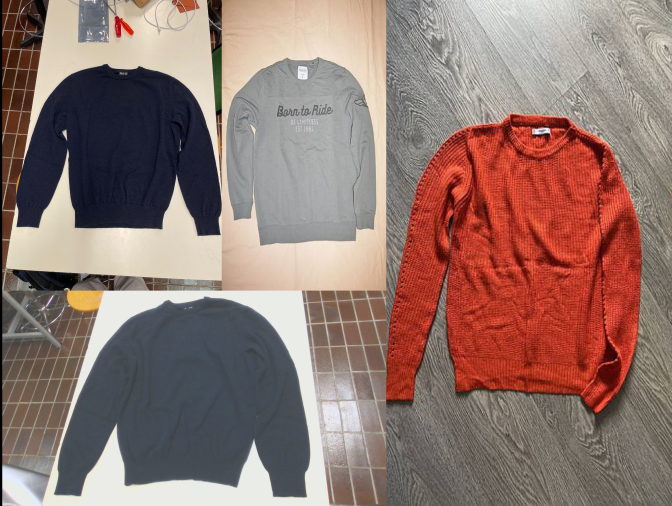
\includegraphics[width=0.8\linewidth]{figures/dataset.png}
        \caption{Immagini Presenti nel Dataset}
        \label{fig:dataset}
    \end{minipage}\hfill
    \begin{minipage}{0.45\textwidth}
        \centering
        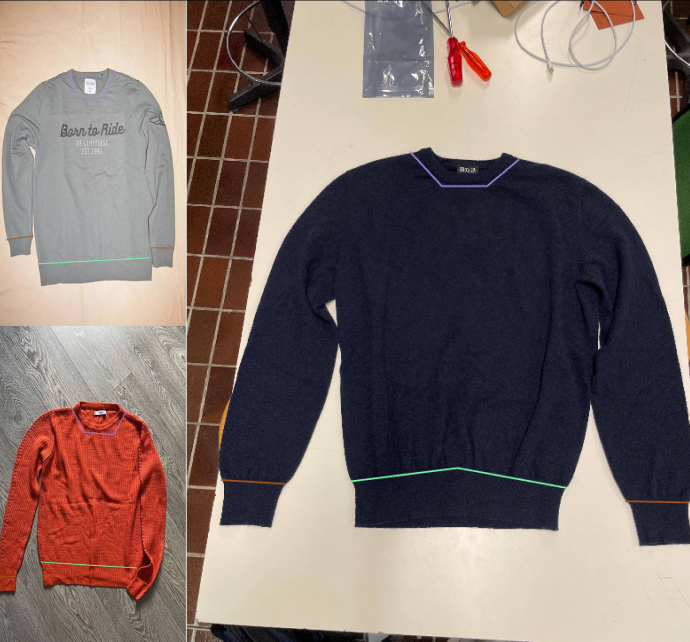
\includegraphics[width=0.7\linewidth]{figures/etichette.png}
        \caption{Immagini Etichettate}
        \label{fig:etichette}
    \end{minipage}
\end{figure}

\section{Architettura YOLOv8-seg Nano}

La scelta del modello è ricaduta su \textbf{YOLOv8-seg Nano (YOLOv8n-seg)}, la versione più leggera e veloce della famiglia Ultralytics YOLOv8 dedicata alla segmentazione delle istanze.

Questa scelta è motivata dalla necessità di operare in tempo reale su hardware embedded, come la Jetson Orin Nano, dove le risorse computazionali e la memoria sono limitate. Nonostante le dimensioni ridotte, l'architettura YOLOv8n-seg garantisce un ottimo compromesso tra velocità (FPS) e accuratezza (mAP).

Caratteristiche principali dell'architettura:
\begin{itemize}
    \item \textbf{Backbone}: Una versione ottimizzata di CSPDarknet53 per l'estrazione delle feature.
    \item \textbf{Neck}: Utilizzo di PANet (Path Aggregation Network) per migliorare la fusione delle feature a diverse scale.
    \item \textbf{Head}: Decoupled Head per la classificazione e la regressione dei box, integrata con un ramo dedicato alla generazione delle maschere di segmentazione tramite prototipi.
\end{itemize}

L'addestramento è stato eseguito per 30 epoche con una dimensione delle immagini di entry a 640x640 pixel, utilizzando l'ottimizzatore SGD e una funzione di loss che combina box loss, class loss e mask loss. Successivamente sono riportate immagini relative alla validazione di alcuni batch di immagini.

\begin{figure}[h!]
    \centering
    \begin{minipage}{0.45\textwidth}
        \centering
        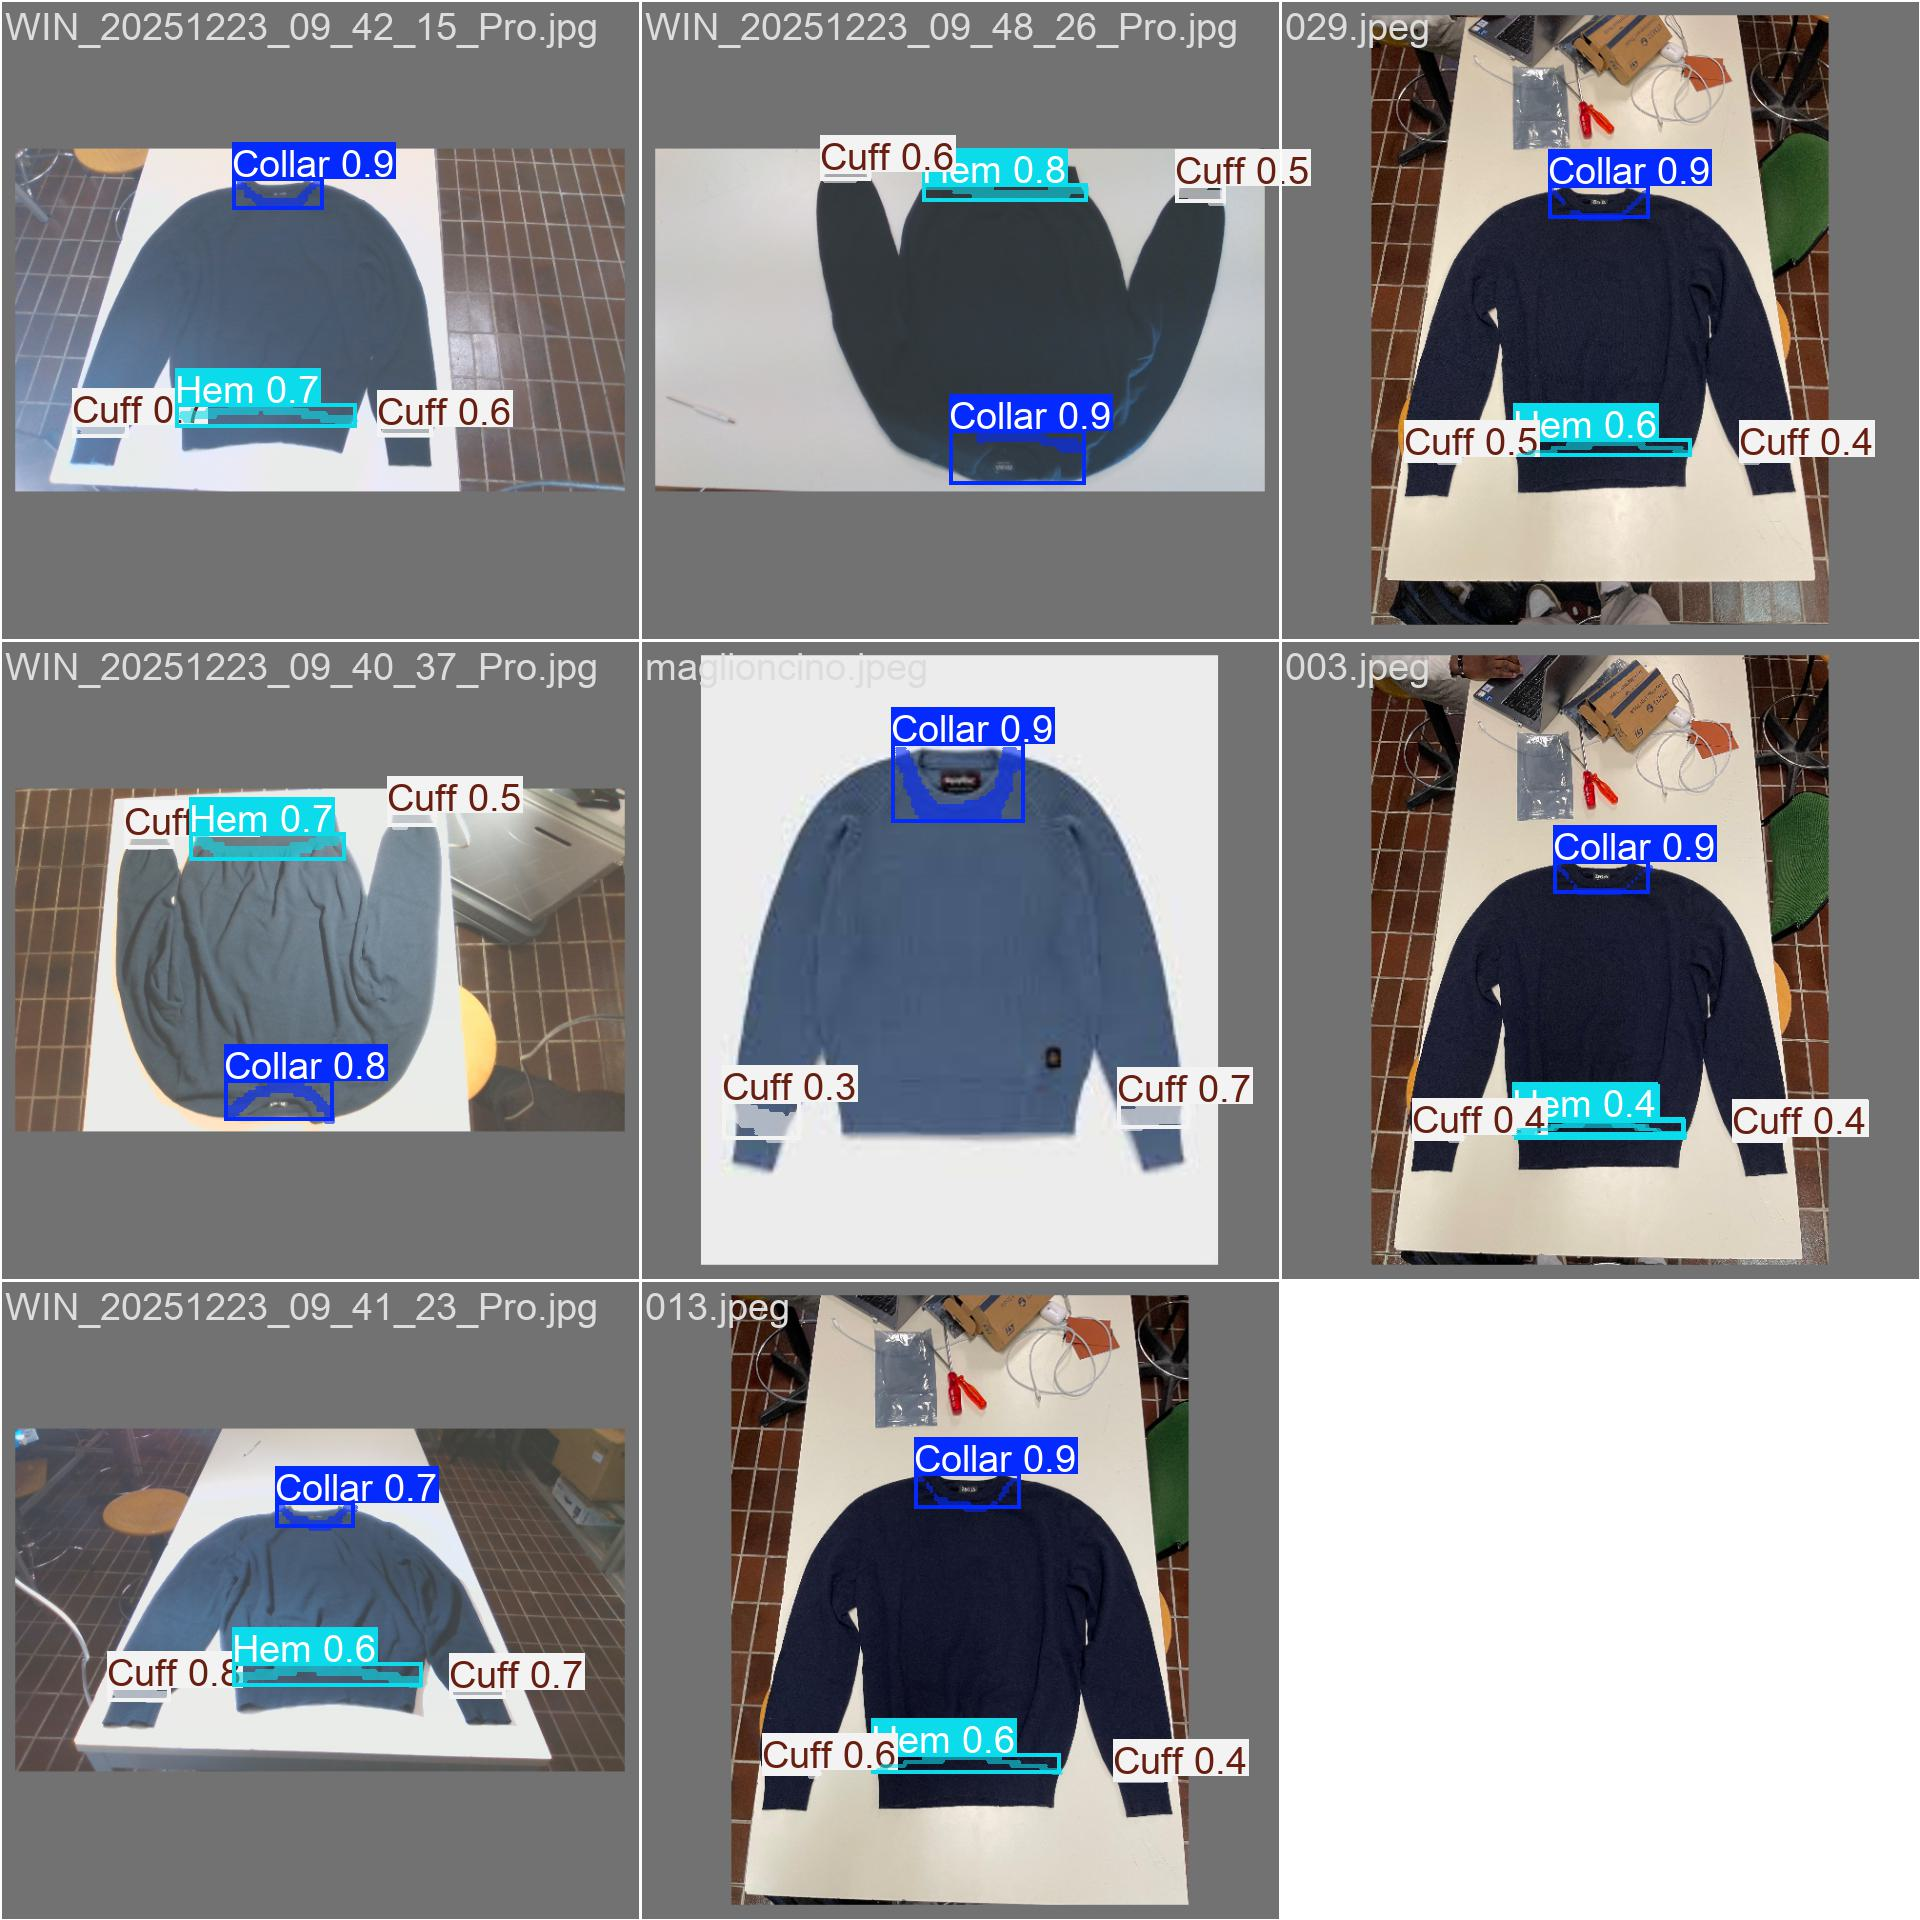
\includegraphics[width=0.9\linewidth]{figures/val_batch1_pred.jpg}
        \caption{Validazione batch 0}
        \label{fig:validazione}
    \end{minipage}\hfill
    \begin{minipage}{0.45\textwidth}
        \centering
        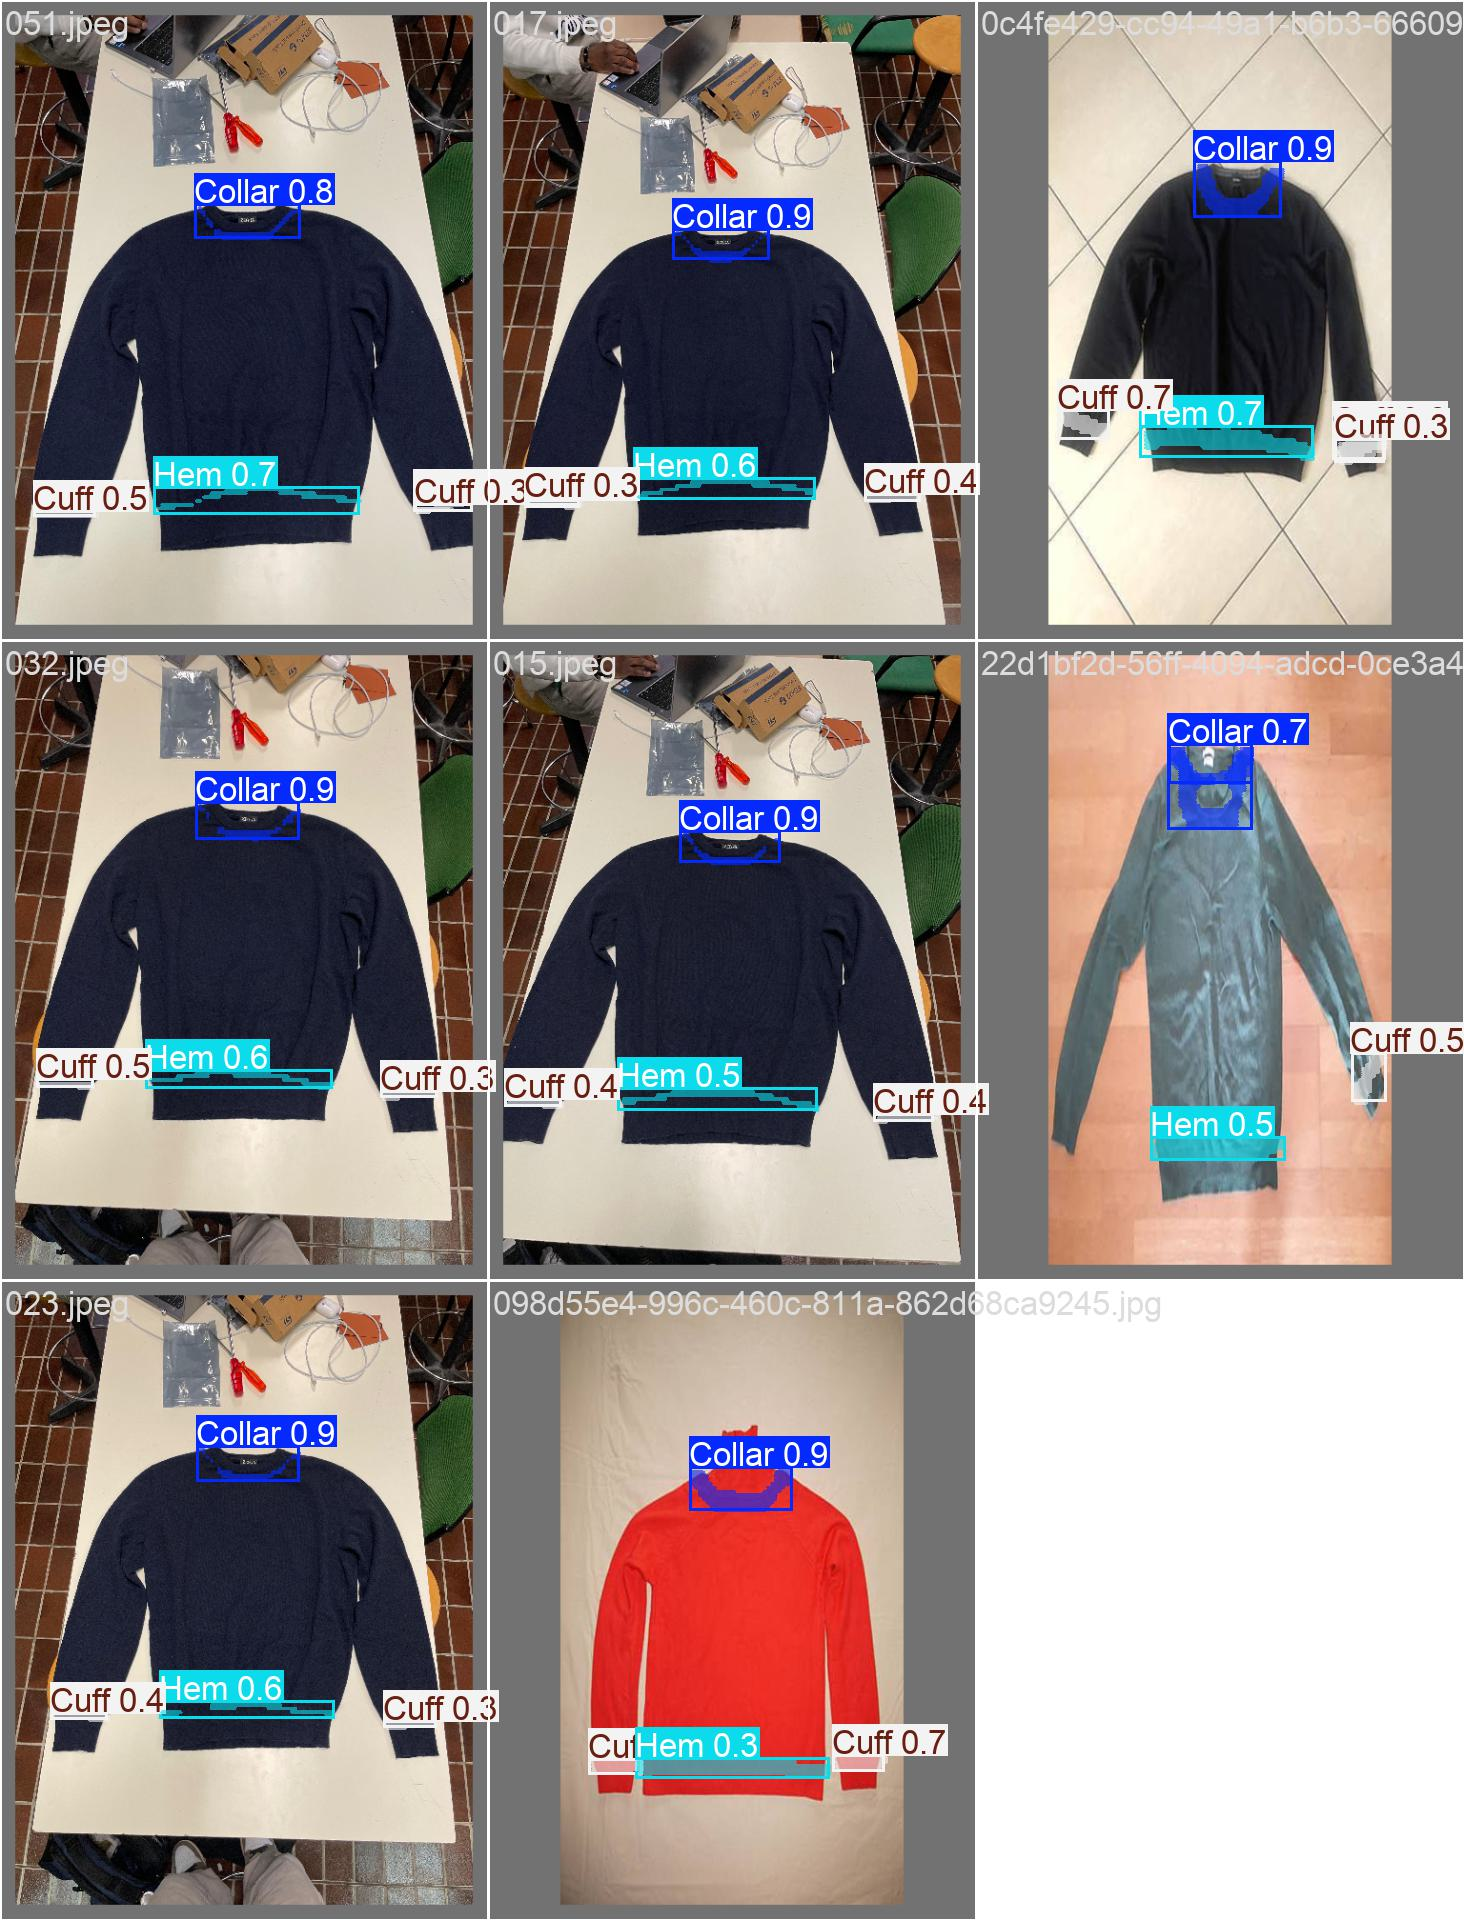
\includegraphics[width=0.7\linewidth]{figures/val_batch2_pred.jpg}
        \caption{Validazione batch 1}
        \label{fig:placeholder}
    \end{minipage}
\end{figure}
\newpage
\section{Valutazione del Modello}

Per valutare le prestazioni della rete YOLOv8n-seg, sono state utilizzate le metriche standard per la segmentazione di istanze. In particolare, sono stati monitorati la Precision, la Recall e la media della precisione media (mAP) sia per i bounding box (rilevamento) che per le maschere (segmentazione).

I risultati ottenuti al termine dell'addestramento sono riassunti nella seguente tabella:

\begin{table}[h]
\centering
\begin{tabular}{|l|c|c|c|}
\hline
\textbf{Metrica} & \textbf{Precision} & \textbf{Recall} & \textbf{mAP@50} \\ \hline
\textbf{Box (Detection)} & 85.4\% & 85.0\% & 90.3\% \\ \hline
\textbf{Mask (Segmentation)} & 65.4\% & 60.7\% & 56.8\% \\ \hline
\end{tabular}
\caption{Metriche di performance del modello YOLOv8n-seg su validation set.}
\label{tab:metrics}
\end{table}

L'elevato valore di mAP@50 per i box (90.3\%) indica un'ottima capacità del modello di localizzare correttamente le zone di interesse. La metrica mAP@50 per le maschere (56.8\%) risulta inferiore, riflettendo la complessità intrinseca della segmentazione di elementi sottili come cuciture e bordi, ma rimane comunque adeguata per l'estrazione della linea media necessaria alla manipolazione.
\\
Successivamente sono riportati i grafici di Precision, Recall dei Box e delle Mask, insieme alla Matrice di confusione normalizzata.
\\\\
\begin{figure}[h]
    \centering
    \makebox[\textwidth][c]{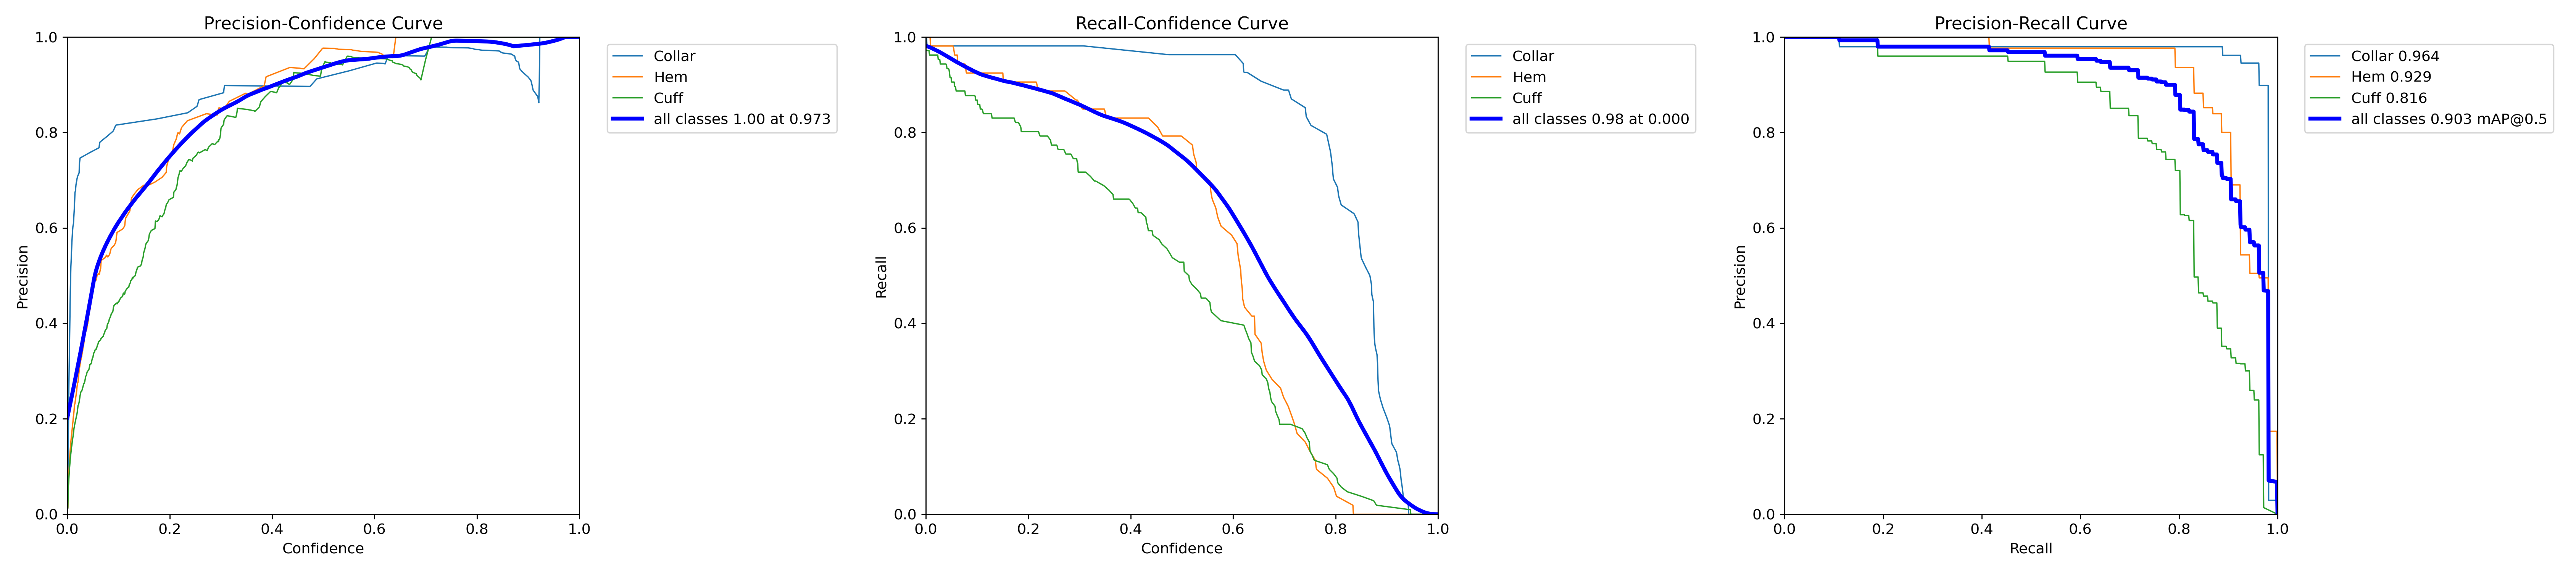
\includegraphics[width=1.2\textwidth]{figures/PR-Box.png}}
    \caption{Box Precision, Recall Confidence e Precision-Recall Curve }
    \label{fig:box}
\end{figure}
\begin{figure}[h]
    \centering
    \makebox[\textwidth][c]{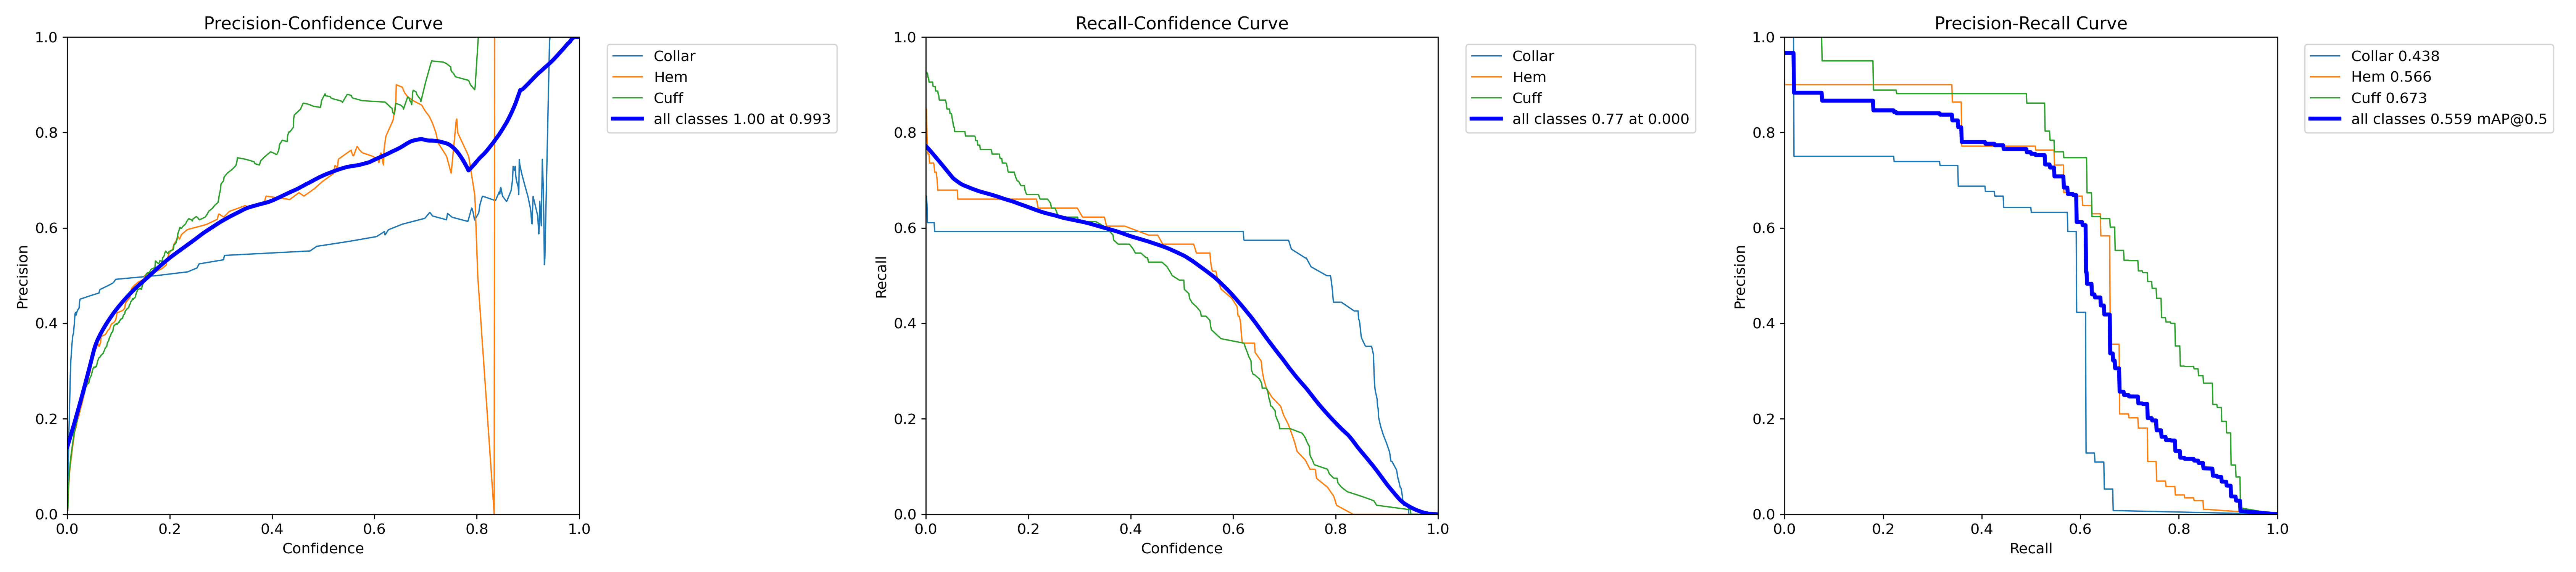
\includegraphics[width=1.2\textwidth]{figures/PR-Mask.png}}
    \caption{Mask Precision, Recall Confidence e Precision-Recall Curve }
    \label{fig:mask}
\end{figure}
\begin{figure}[H]
    \centering
    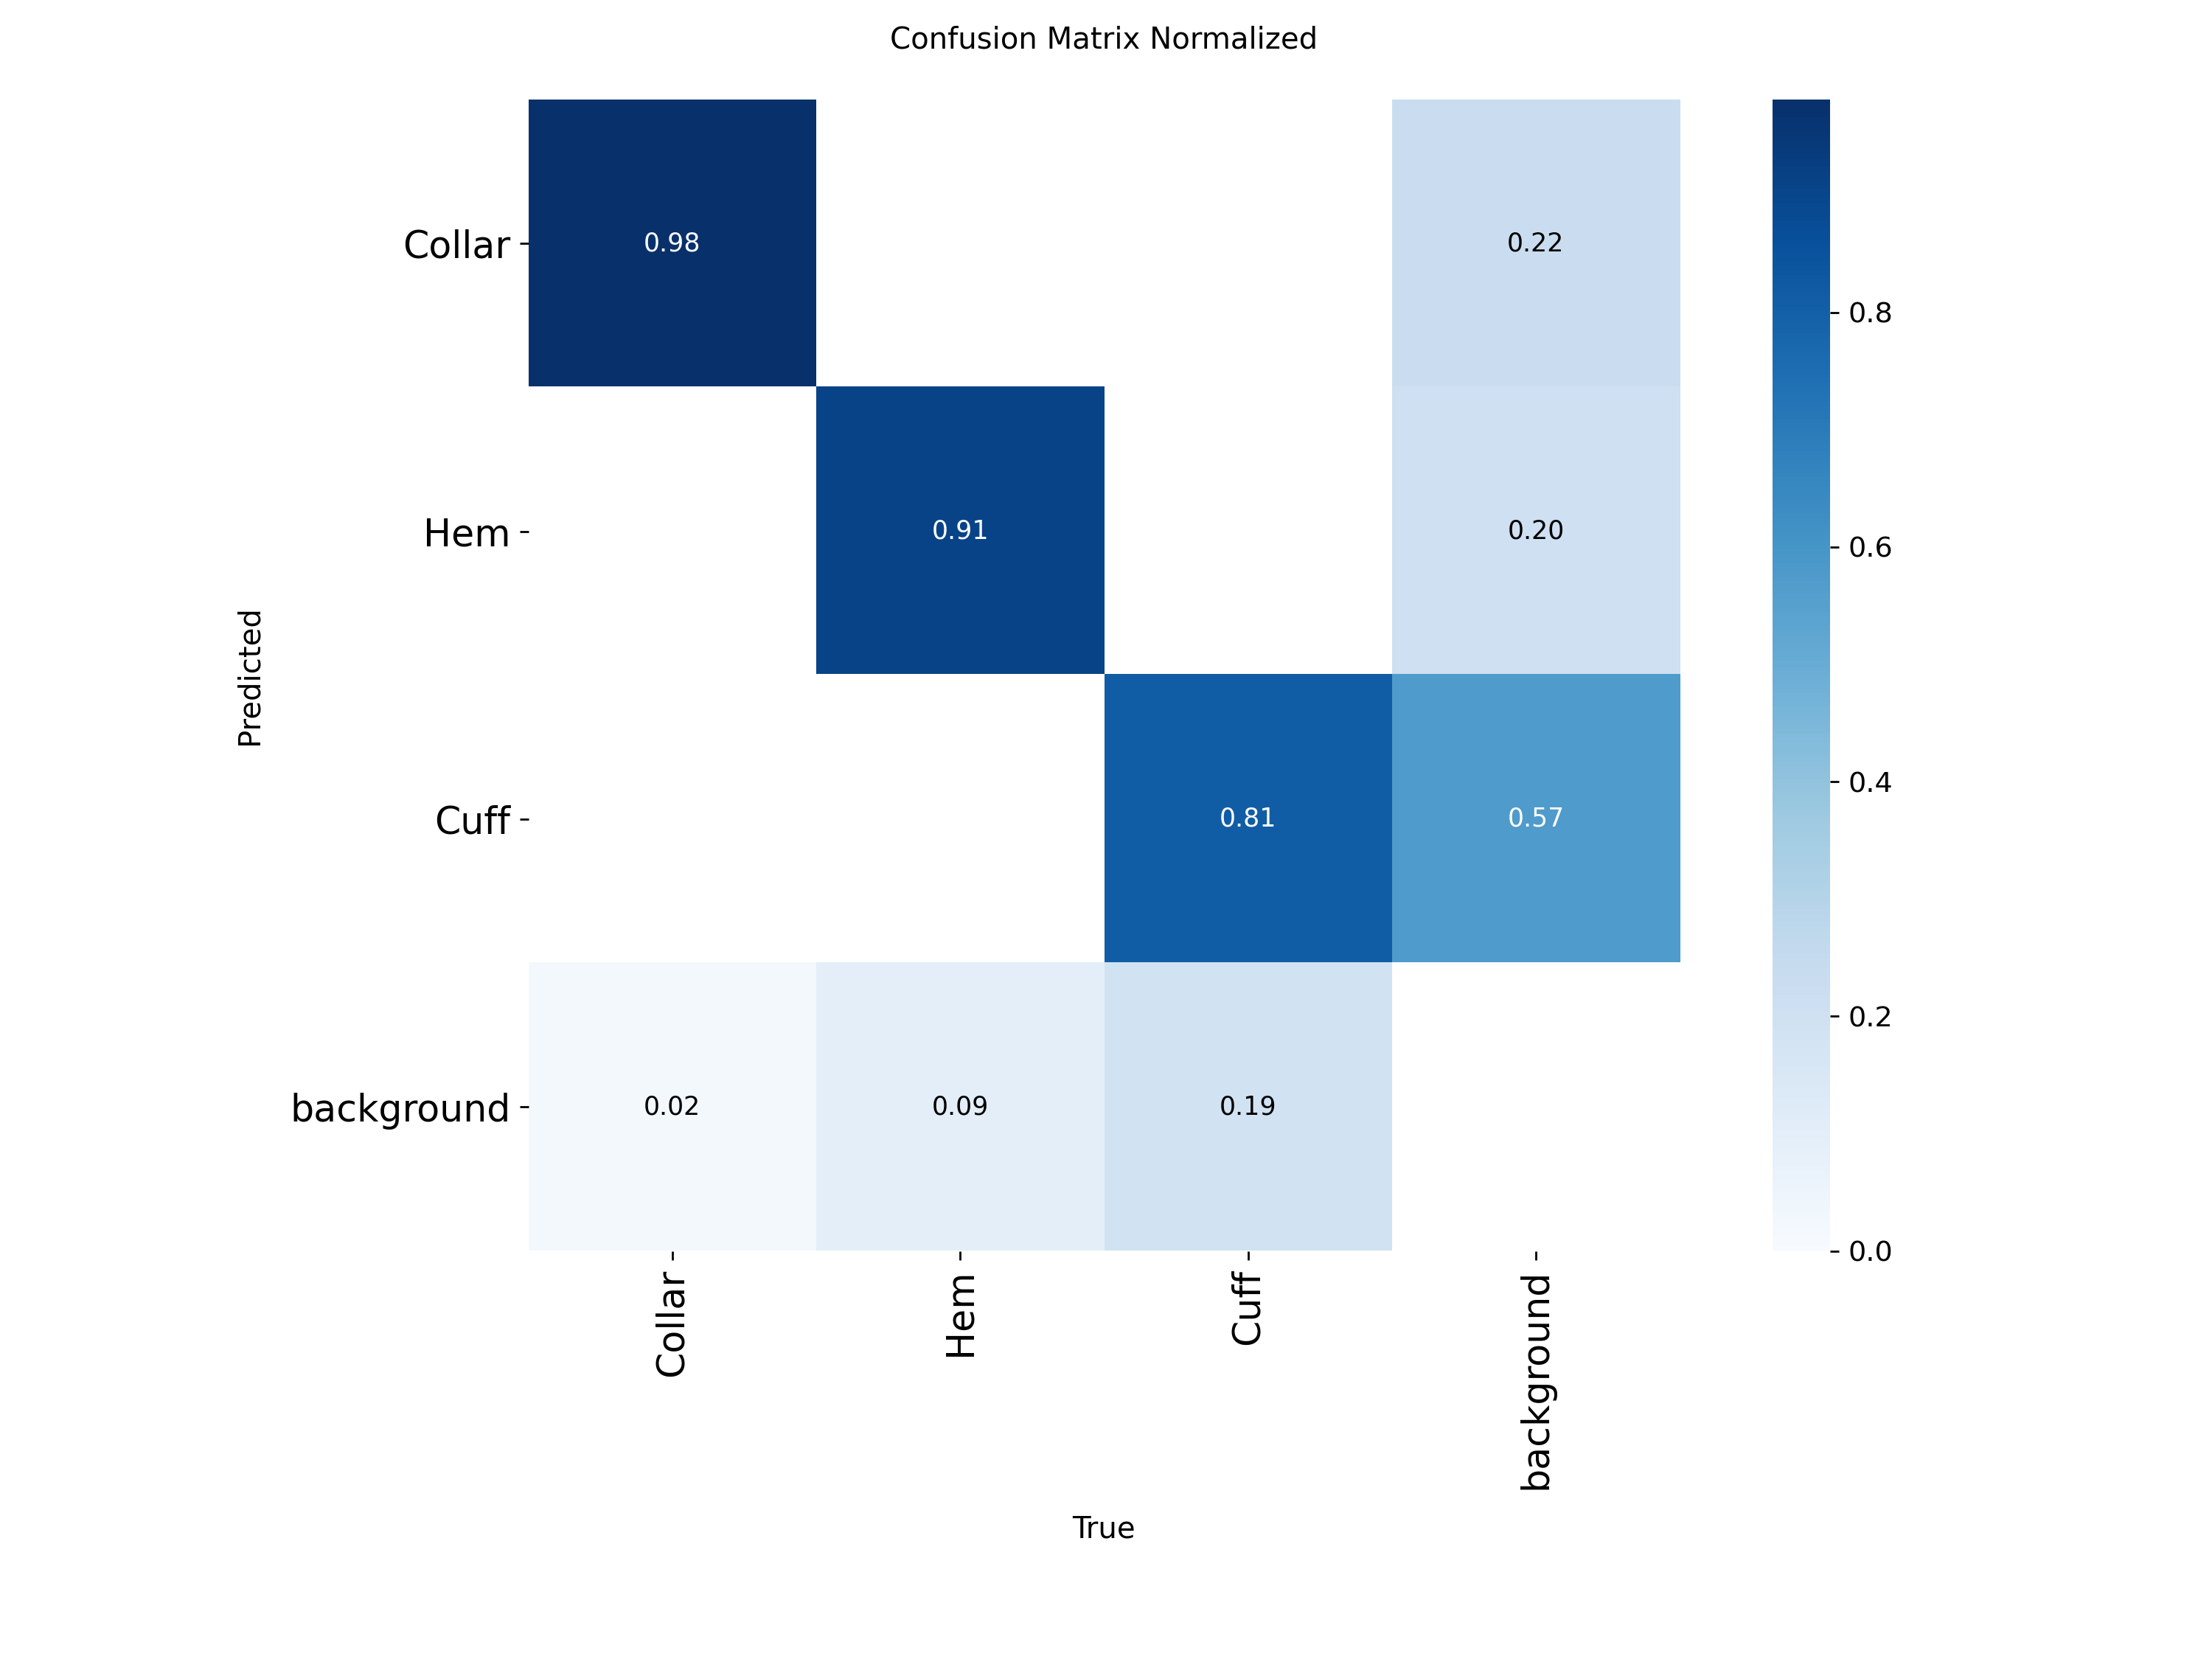
\includegraphics[width=1\linewidth]{figures/confusion_matrix_normalized.png}
    \caption{Matrice di confusione normalizzata}
    \label{fig:confusion matrix}
\end{figure}

\newpage
\section{Estrazione Coordinate}

Una volta ottenute le maschere dalle predizioni del modello, viene applicato un algoritmo di estrazione geometrica per individuare i punti critici.

L'algoritmo segue i seguenti passaggi:
\begin{enumerate}
    \item \textbf{Filtraggio Maschere}: Se più istanze della stessa classe vengono rilevate, viene mantenuta solo quella con il punteggio di confidenza più elevato, applicando un filtraggio basato su Intersection over Union (IoU) per eliminare sovrapposizioni spurie.
    \item \textbf{Y-Averaging (Calcolo Linea Media)}: Per ogni coordinata $x$ lungo la maschera, viene calcolata la media dei valori $y$ dei pixel appartenenti alla maschera. Questo permette di individuare la "linea centrale" dell'elemento (ad esempio, il centro della curva del colletto) ignorando lo spessore del bordo.
    \item \textbf{Campionamento Punti}:
    \begin{itemize}
        \item Per il \textbf{Collar} e l' \textbf{Hem}, vengono estratti $N$ punti equidistanti lungo l'asse $x$ per rappresentare la curvatura della cucitura.
        \item Per i \textbf{Cuff}, vengono estratti unicamente i punti estremi (inizio e fine) per definire l'orientamento del polsino.
    \end{itemize}
    \item \textbf{Proiezione 3D}: Per ogni punto $(x, y)$ estratto nell'immagine 2D, viene recuperato il valore di profondità $z$ dal frame depth sincronizzato. Sfruttando i parametri intrinseci della camera, le coordinate pixel vengono infine trasformate in coordinate tridimensionali nel sistema di riferimento del robot.
\end{enumerate}

Le coordinate estratte vengono salvate in formato JSON per essere utilizzate dal modulo di pianificazione delle traiettorie.

\begin{figure}[h!]
    \centering
    \begin{minipage}{0.45\textwidth}
        \centering
        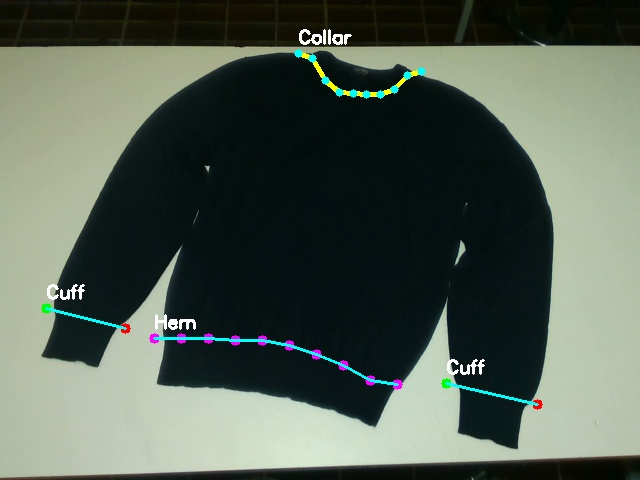
\includegraphics[width=0.8\linewidth]{figures/inference_result_depth.jpg}
        \caption{Estrazione dei punti}
        \label{fig:punti}
    \end{minipage}\hfill
    \begin{minipage}{0.45\textwidth}
        \centering
        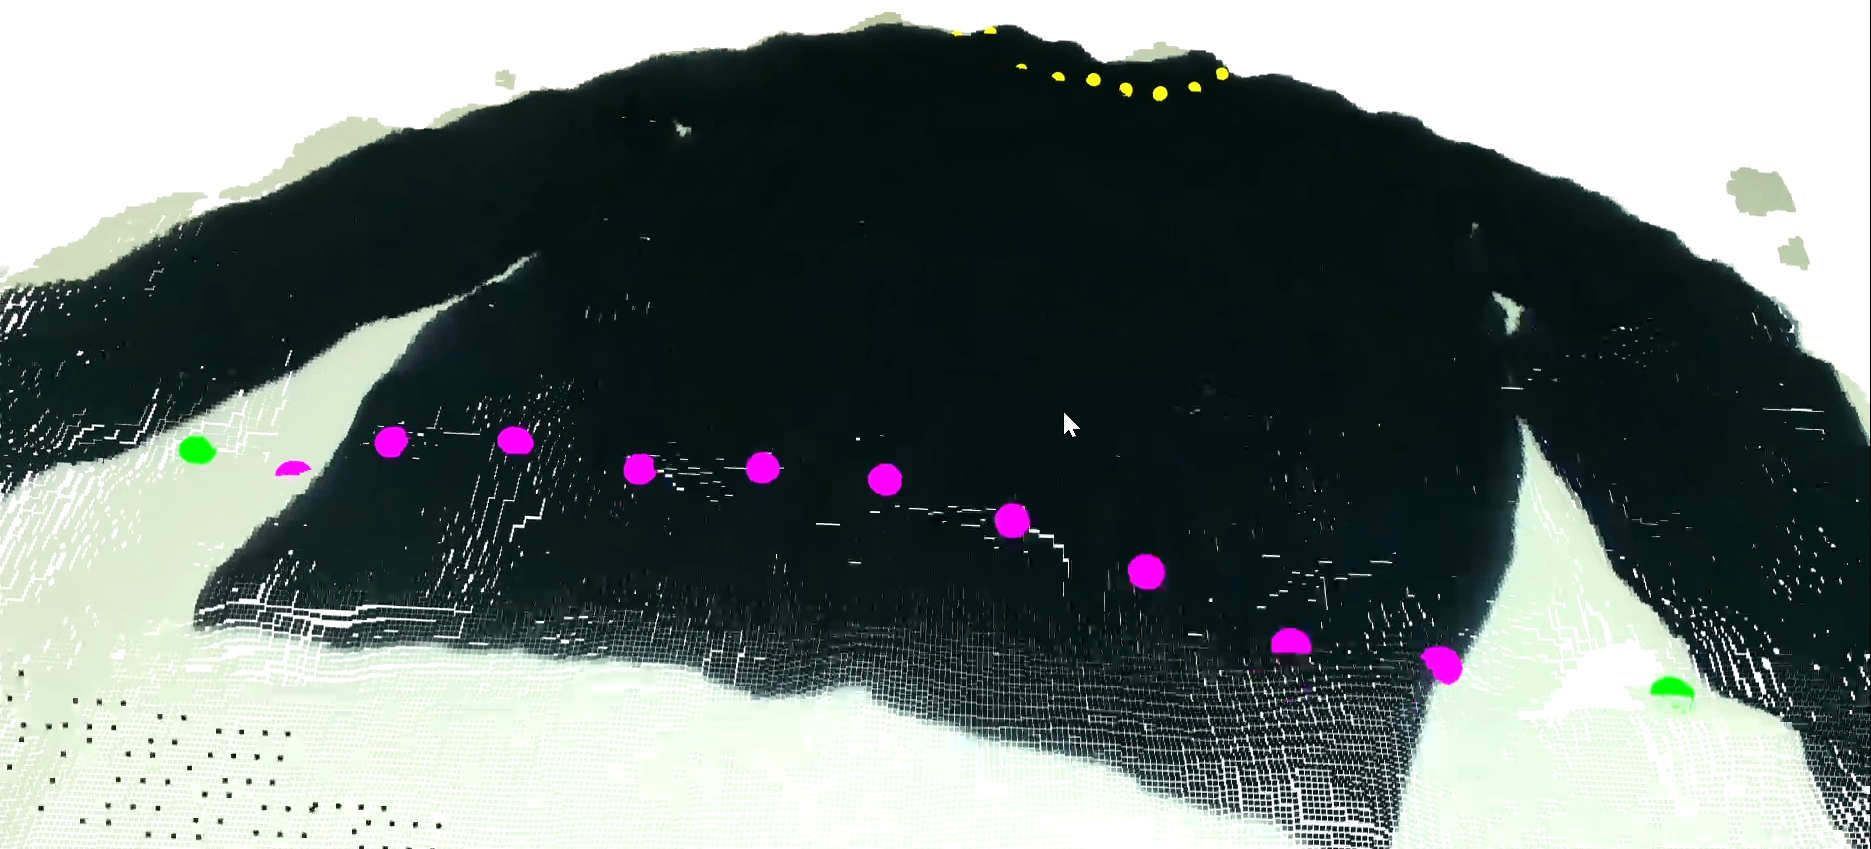
\includegraphics[width=1\linewidth]{figures/ricostruzione3d.png}
        \caption{Ricostruzione 3D dei punti estratti}
        \label{fig:ricostruzione 3D}
    \end{minipage}
\end{figure}

\newpage
Esempio di JSON:
\begin{verbatim}
{
    "Cuff": [
        {
            "start": [
                x, y, z
            ],
            "end": [
                x, y, z
            ]
        },
        {
            "start": [
                x, y, z
            ],
            "end": [
                x, y, z
            ]
        }
    ],
    "Hem": [
        {
            "points": [
                [
                    x, y, z
                ],
                ...
            ]
        }
    ],
    "Collar": [
        {
            "points": [
                [
                    x, y, z
                ],
                ...
            ]
        }
    ]
}
\end{verbatim}

\chapter{Architettura ROS~2}
\label{chap:architettura_ros2}

Di seguito viene descritta l'architettura del sistema di controllo implementato in ROS~2, evidenziando i principali nodi e le loro interazioni. L'architettura è stata progettata per garantire modularità, scalabilità e facilità di integrazione sia con il sistema di simulazione in Unity che con il robot reale.

\section{Architettura per Unity}

L'architettura del sistema di simulazione in Unity è composta da diversi componenti principali, ognuno dei quali svolge un ruolo specifico nell'integrazione con ROS~2 e nella simulazione del comportamento del robot. I principali componenti includono:

\begin{figure}[H]
    \centering
    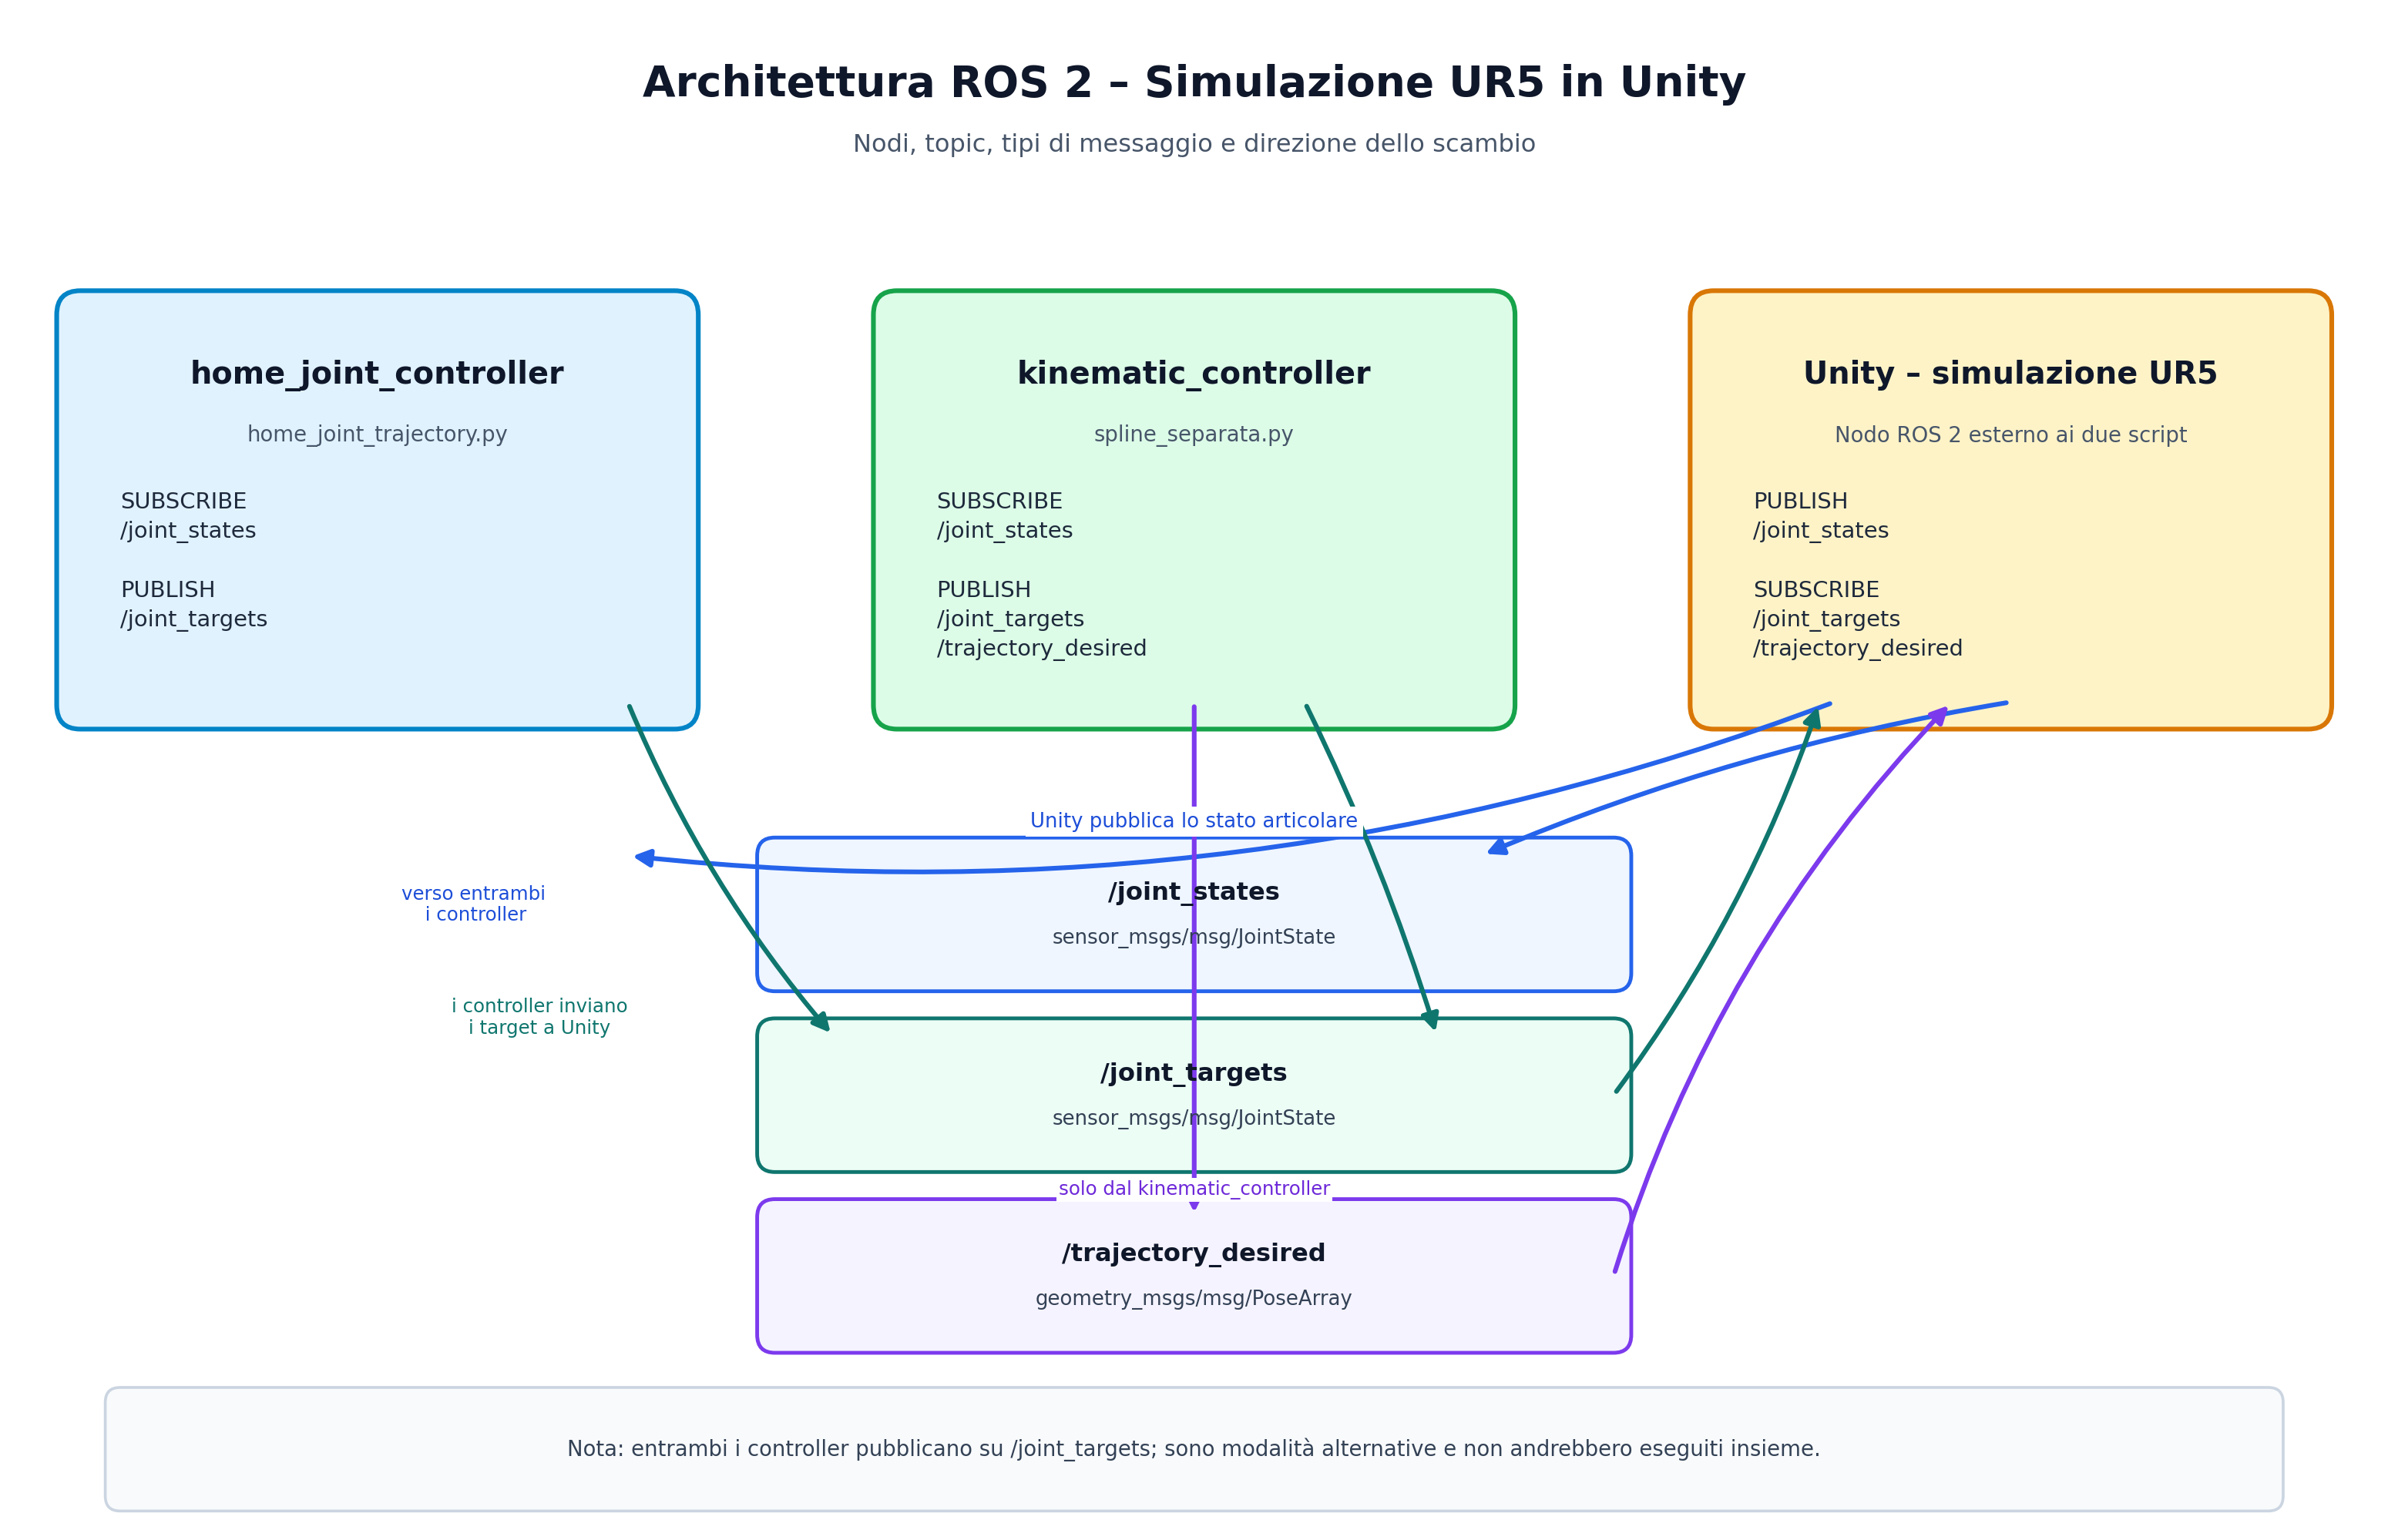
\includegraphics[width=1.0\linewidth]{figures/ros/schema_ros_unity.png}
    \caption{Architettura ROS~2 per Unity}
    \label{fig:architettura_ros2_per_unity}
\end{figure}

\newpage
\section{Architettura per il robot reale}

L'architettura del sistema di controllo per il robot reale si basa sulla struttura precedente ma con alcune modifiche per adattarsi alle specifiche del robot e alle sue capacità hardware.
Nello specifico, invece di utilizzare messaggi su topic per la comunicazione con il robot, si fa uso di action server e action client per gestire le richieste di movimento e le risposte del robot in modo più efficiente, coerentemente con il driver e controller dell'UR5.
Rispetto al caso precedente, c'è inoltre una trasformazione statica dalla camera al \texttt{wrist\_2\_link} che permette di allineare correttamente le coordinate del sistema di riferimento della camera con quelle del robot tramite poi l'utilizzo di \textit{TF}.
I principali componenti includono:

\begin{figure}[H]
    \centering
    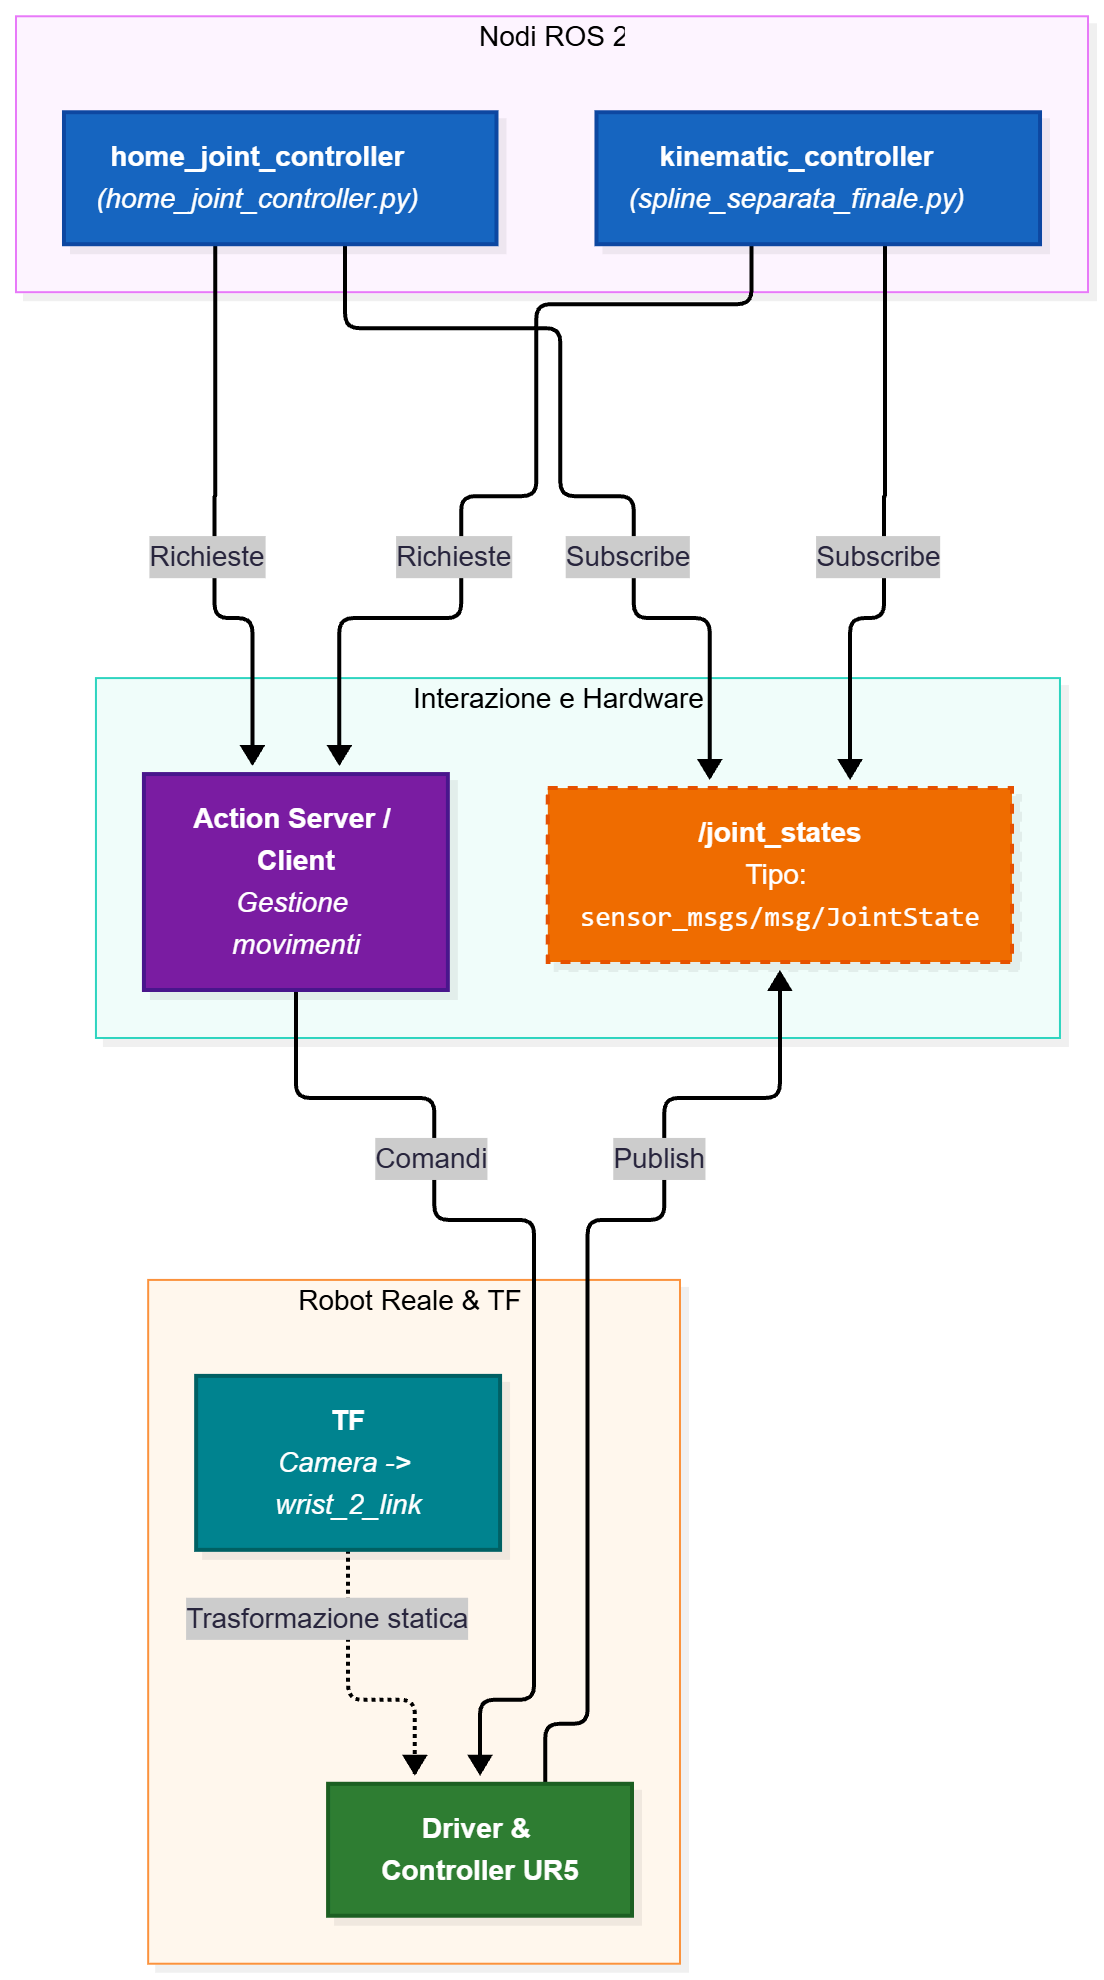
\includegraphics[width=0.5\linewidth]{figures/ros/schema_ros_reale.png}
    \caption{Architettura ROS~2 Robot reale}
    \label{fig:architettura_rosrobot_unity}
\end{figure}

\section{Architettura per il robot reale - Launcher automatico}

Questa versione dell'architettura è stata progettata per semplificare l'avvio del sistema di controllo del robot reale, automatizzando il processo di lancio dei nodi necessari e garantendo una configurazione coerente e ripetibile.
Il launcher automatico consente di avviare tutti i componenti del sistema con un singolo comando, comprendendo la traiettoria per la \textit{home\_position}, lo scatto della foto, l'inferenza del modello e la traiettoria per i punti estratti.
In questo modo si elimina la necessità di avviare manualmente ogni nodo e di riportare manualmente le coordinate dei punti estratti, riducendo il rischio di errori e migliorando l'efficienza complessiva del processo di controllo del robot.

\chapter{Simulazione del sistema robotico in Unity}

Prima della sperimentazione sul robot reale è stato sviluppato un ambiente di simulazione in Unity, con l'obiettivo di validare l'intera pipeline di controllo e verificare il comportamento del sistema in un ambiente virtuale. La simulazione ha permesso di testare il modello cinematico del manipolatore, la comunicazione con ROS~2, la simulazione del sensore di visione e l'interazione con un capo di abbigliamento deformabile, riducendo tempi e rischi durante la fase di sviluppo.

\section{Importazione del modello del robot}

Il manipolatore utilizzato è un Universal Robots UR5, il cui modello è stato importato in Unity a partire dalla descrizione URDF (Unified Robot Description Format). L'importazione è stata effettuata mediante il pacchetto \textit{Unity Robotics Hub}, che consente di convertire automaticamente la struttura del robot in una gerarchia di oggetti Unity mantenendo la relazione cinematica tra i vari link.

Durante l'importazione vengono creati automaticamente tutti i collegamenti tra i link del robot, rispettando la struttura descritta nel file URDF. Ogni giunto rotazionale viene convertito in un componente \textit{ArticulationBody}, introdotto da Unity per la simulazione fisica dei robot. Tale componente implementa un modello dinamico basato sul motore fisico PhysX e permette di simulare correttamente vincoli articolari, masse, inerzie e limiti meccanici.

I giunti del robot risultano quindi organizzati secondo la stessa catena cinematica presente sul manipolatore reale:

\begin{center}
\texttt{base\_link} $\rightarrow$
\texttt{shoulder\_link} $\rightarrow$
\texttt{upper\_arm\_link} $\rightarrow$
\texttt{forearm\_link} $\rightarrow$
\texttt{wrist\_1\_link} $\rightarrow$
\texttt{wrist\_2\_link} $\rightarrow$
\texttt{wrist\_3\_link}.
\end{center}

Ciò permette di utilizzare lo stesso modello cinematica impiegato nel sistema reale, garantendo una corrispondenza diretta tra simulazione ed esperimento.

\section{Simulazione del capo di abbigliamento}

Per simulare il comportamento deformabile del maglione è stato utilizzato il plugin Obi Cloth, una libreria sviluppata per Unity che implementa un modello fisico basato su particelle (Position Based Dynamics).

A differenza della fisica standard di Unity, Obi Cloth consente di rappresentare materiali tessili caratterizzati da elevate deformazioni, pieghe e interazioni con corpi rigidi. Ogni vertice della mesh del maglione viene convertito in una particella fisica collegata alle particelle vicine mediante vincoli elastici, consentendo di simulare realisticamente il comportamento del tessuto durante le deformazioni.

Il modello tridimensionale del maglione è stato importato come mesh OBJ e successivamente convertito in un oggetto Obi Cloth.

\section{Simulazione della telecamera}

Per riprodurre il comportamento della Intel RealSense D453i è stata installata una telecamera virtuale come figlia del link \texttt{wrist\_2\_link}, in modo che seguisse rigidamente tutti i movimenti del manipolatore.

La telecamera virtuale è stata configurata con gli stessi parametri principali della camera reale, quali campo visivo, risoluzione e posizione relativa rispetto all'end-effector.

È stato inoltre sviluppato uno script C\# dedicato alla simulazione della RealSense che permette di acquisire l'immagine RGB. Le acquisizioni vengono quindi salvate sul disco in modo da poter essere elaborate successivamente dalla rete neurale utilizzata per l'estrazione dei punti caratteristici del capo.

\section{Comunicazione tra Unity e ROS 2}

L'ambiente Unity è stato integrato con ROS~2 Humble mediante il pacchetto ROS-TCP-Connector sviluppato da Unity Robotics.

Il pacchetto implementa una connessione TCP/IP tra Unity e ROS~2, consentendo lo scambio bidirezionale di messaggi in tempo reale.

Nel sistema sviluppato il nodo ROS pubblica continuamente sul topic dedicato gli angoli dei giunti desiderati del robot.

Unity sottoscrive tale topic mediante uno script C\#, che converte il messaggio ROS ricevuto nei corrispondenti valori degli \textit{ArticulationBody}. Ogni giunto viene quindi aggiornato modificando direttamente il parametro \textit{xDrive.target}, che rappresenta la posizione angolare desiderata del giunto.

Questo approccio permette di utilizzare lo stesso nodo di controllo sviluppato per il robot reale senza apportare modifiche all'algoritmo di pianificazione della traiettoria. Dal punto di vista del software ROS, infatti, il simulatore rappresenta semplicemente un differente attuatore.

\section{Validazione della pipeline}

La simulazione ha consentito di verificare l'intera pipeline sviluppata.

In particolare è stato possibile validare:

\begin{itemize}
    \item il modello cinematico del manipolatore;
    \item la corretta conversione delle coordinate tra i sistemi di riferimento della camera e del robot;
    \item la generazione delle traiettorie dell'end-effector;
    \item la sincronizzazione tra ROS~2 e Unity;
    \item il funzionamento della simulazione della telecamera RGB-D;
    \item l'interazione tra il manipolatore e il maglione.
\end{itemize}

L'utilizzo dell'ambiente virtuale ha consentito di individuare e correggere numerosi problemi relativi ai sistemi di riferimento, alle trasformazioni geometriche e alla comunicazione tra i diversi moduli software prima dell'esecuzione degli esperimenti sul robot reale, riducendo significativamente i tempi di sviluppo e aumentando l'affidabilità complessiva del sistema.

\section{Esecuzione del sistema}

Una volta stabilita la comunicazione tra Unity e ROS~2 mediante il pacchetto \textit{ROS-TCP-Connector}, viene avviata la sequenza operativa del sistema. Il primo nodo eseguito è \textit{home\_joint.py}, il cui compito è portare il manipolatore nella configurazione di \textit{home} precedentemente definita. Tale configurazione è stata scelta in modo da garantire che la telecamera montata sul robot inquadri completamente il maglione, assicurando condizioni di acquisizione ripetibili e una corretta visibilità delle principali caratteristiche del capo.

\begin{figure}[H]
    \centering
    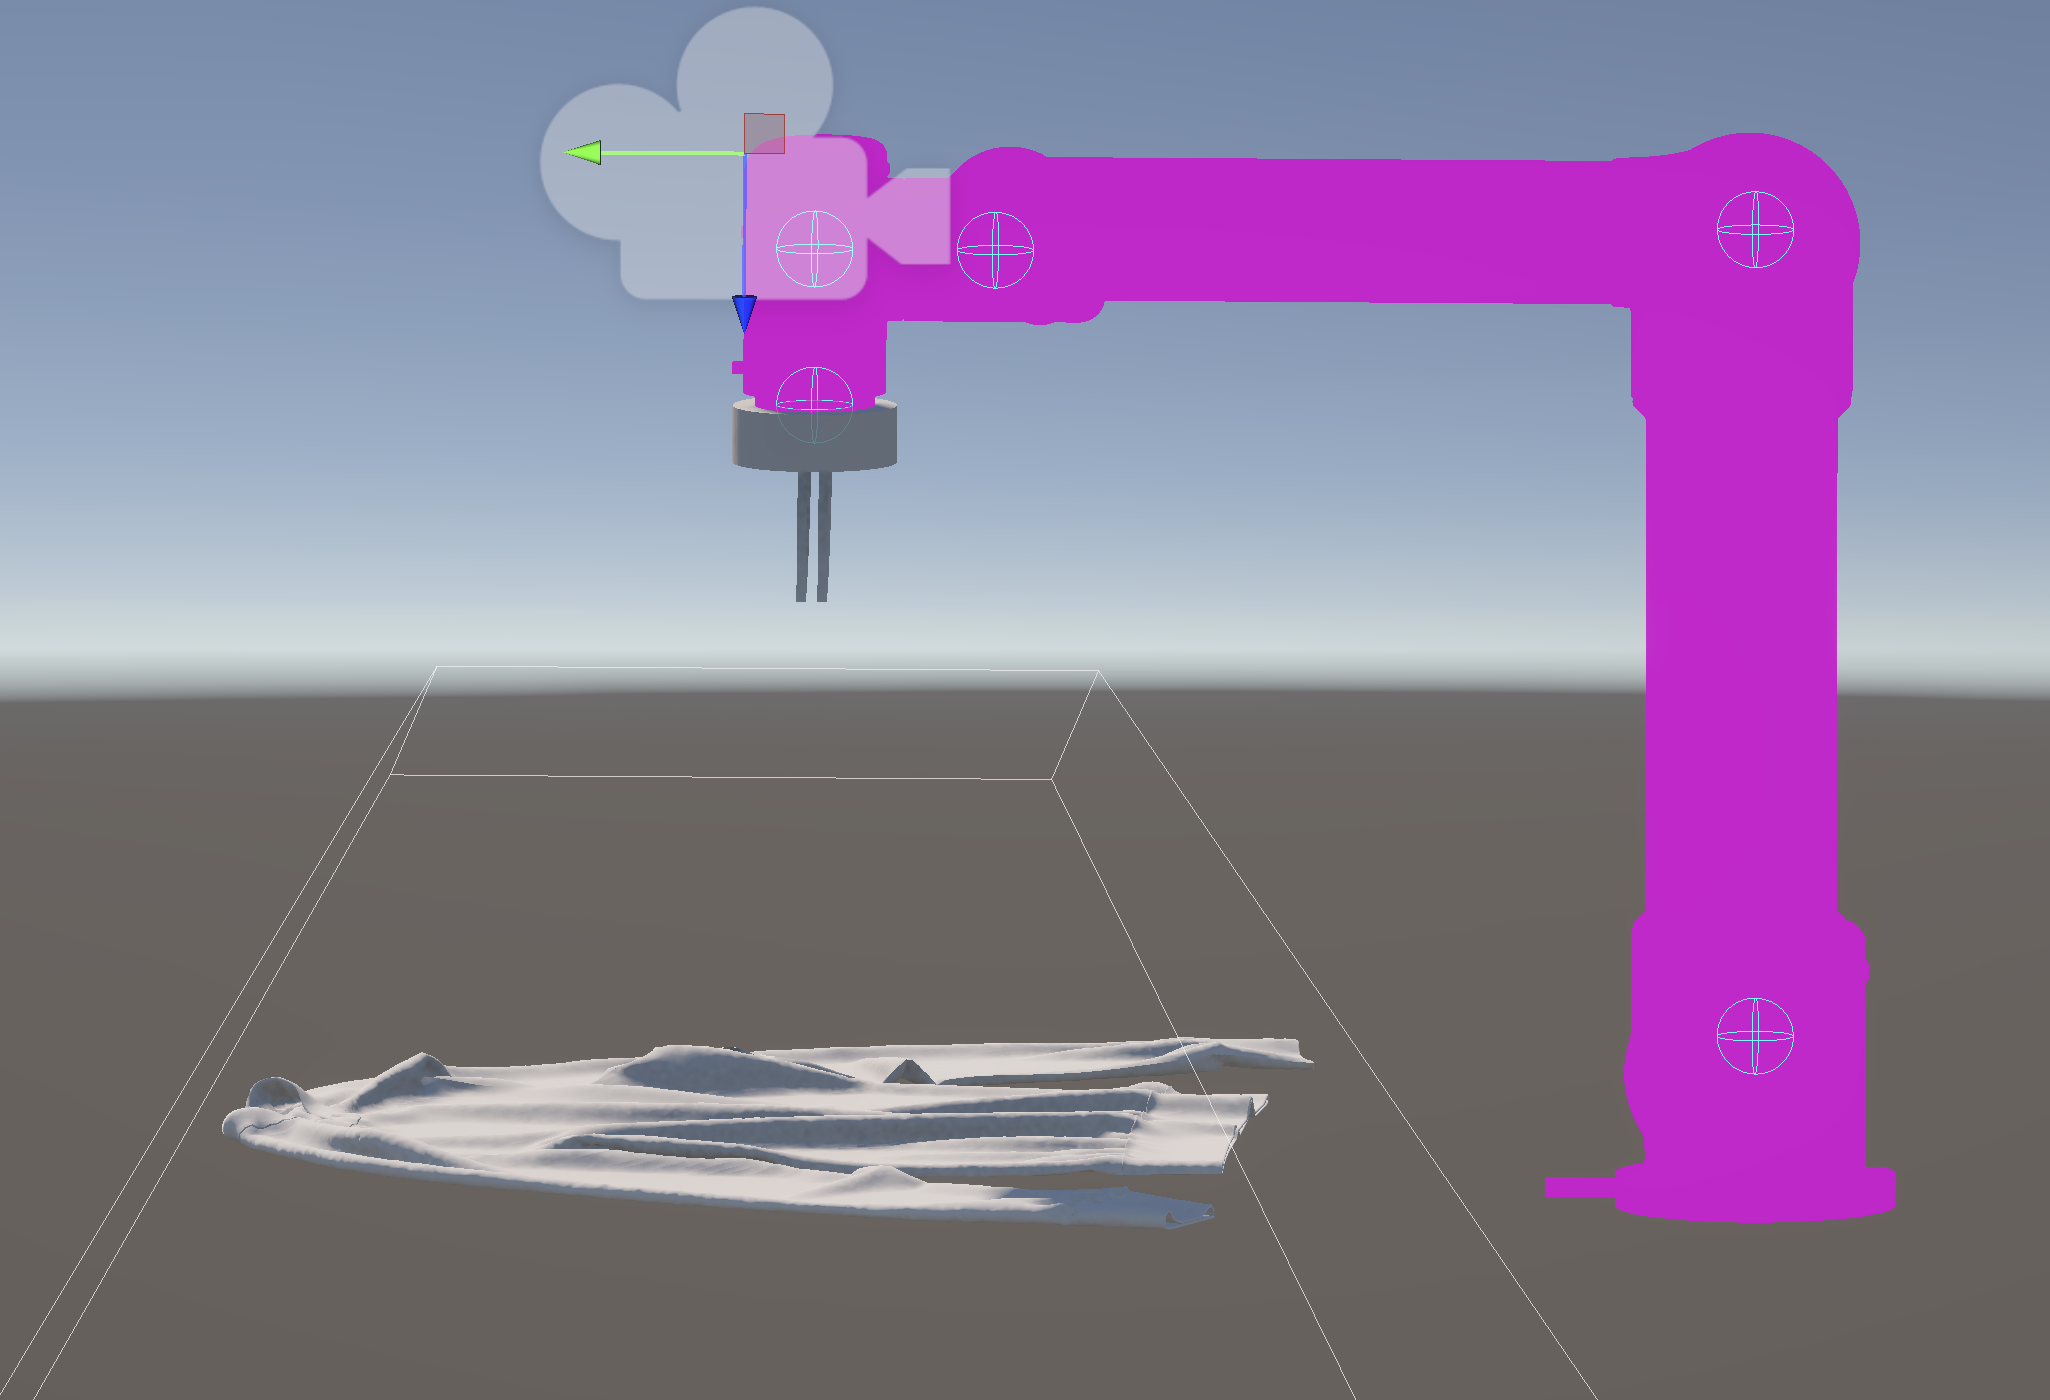
\includegraphics[width=0.75\linewidth]{figures/unity/posizione_home.png}
    \caption{Home Position}
    \label{fig:home position}
\end{figure}

Raggiunta la posizione iniziale, viene acquisita un'immagine RGB del maglione mediante la telecamera simulata. L'immagine viene salvata all'interno della cartella \texttt{Assets} del progetto Unity e successivamente utilizzata come input per la rete neurale sviluppata per l'identificazione dei punti di interesse del capo. In particolare, il modello esegue un'inferenza sull'immagine acquisita ed estrae le coordinate dei punti appartenenti al colletto, ai due polsini e al fondo del maglione, che rappresentano i riferimenti necessari per la generazione della traiettoria di manipolazione.
\begin{figure}[H]
    \centering
    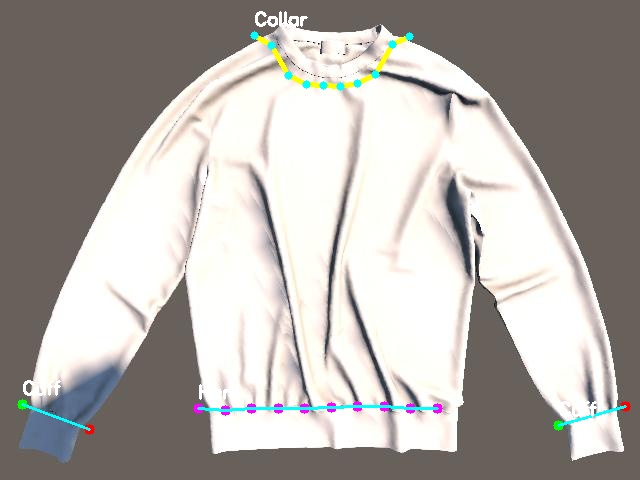
\includegraphics[width=0.75\linewidth]{figures/unity/yolo_inference_unity_result.jpg}
    \caption{Estrazione coordinate tramite rete neurale}
    \label{fig:estrazione coordinate tramite rete neurale}
\end{figure}

Le coordinate prodotte dalla rete neurale vengono quindi elaborate dal nodo \textit{spline\_finale.py}, che costituisce il modulo principale di pianificazione del moto.
I punti vengono presi dallo script python relativi all'inferenza e successivamente inseriti manualmente all'interno nodo precedentemente menzionato.
In una prima fase, i punti vengono convertiti dal sistema di riferimento della telecamera a quello della base del robot mediante opportune trasformazioni geometriche che prevedono l'utilizzo della matrice di trasformazione ricavata da Unity.
Successivamente, il nodo genera una curva spline che interpola i punti estratti, ottenendo una traiettoria continua e sufficientemente regolare da poter essere seguita dal manipolatore.

Per garantire un movimento fluido e privo di brusche variazioni di velocità, la traiettoria geometrica viene parametrizzata temporalmente ed è composta da una serie di profili di velocità trapezoidali che definiscono l'evoluzione temporale del moto dell'end-effector.
A ogni istante di campionamento vengono determinati il riferimento cartesiano desiderato per l'end-effector e la sua posizione attuale, ricavata dallo stato del manipolatore.
Lo stato articolare corrente del manipolatore viene utilizzato per calcolare la posa effettiva dell'end-effector mediante cinematica diretta. Confrontando quest'ultima con la posa desiderata, vengono determinati l'errore di posizione e quello di orientamento.
Il controllo in retroazione integra tali errori nella velocità cartesiana di riferimento, sommando al contributo di velocità pianificata un termine correttivo proporzionale all'errore.
Il Jacobiano del manipolatore viene quindi invertito mediante il metodo Damped Least Squares (DLS), così da poter essere utilizzato per l'ultimo passo della cinematica inversa e ottenere i riferimenti articolari da inviare al robot attraverso i topic ROS~2.

\begin{figure}[H]
    \centering
    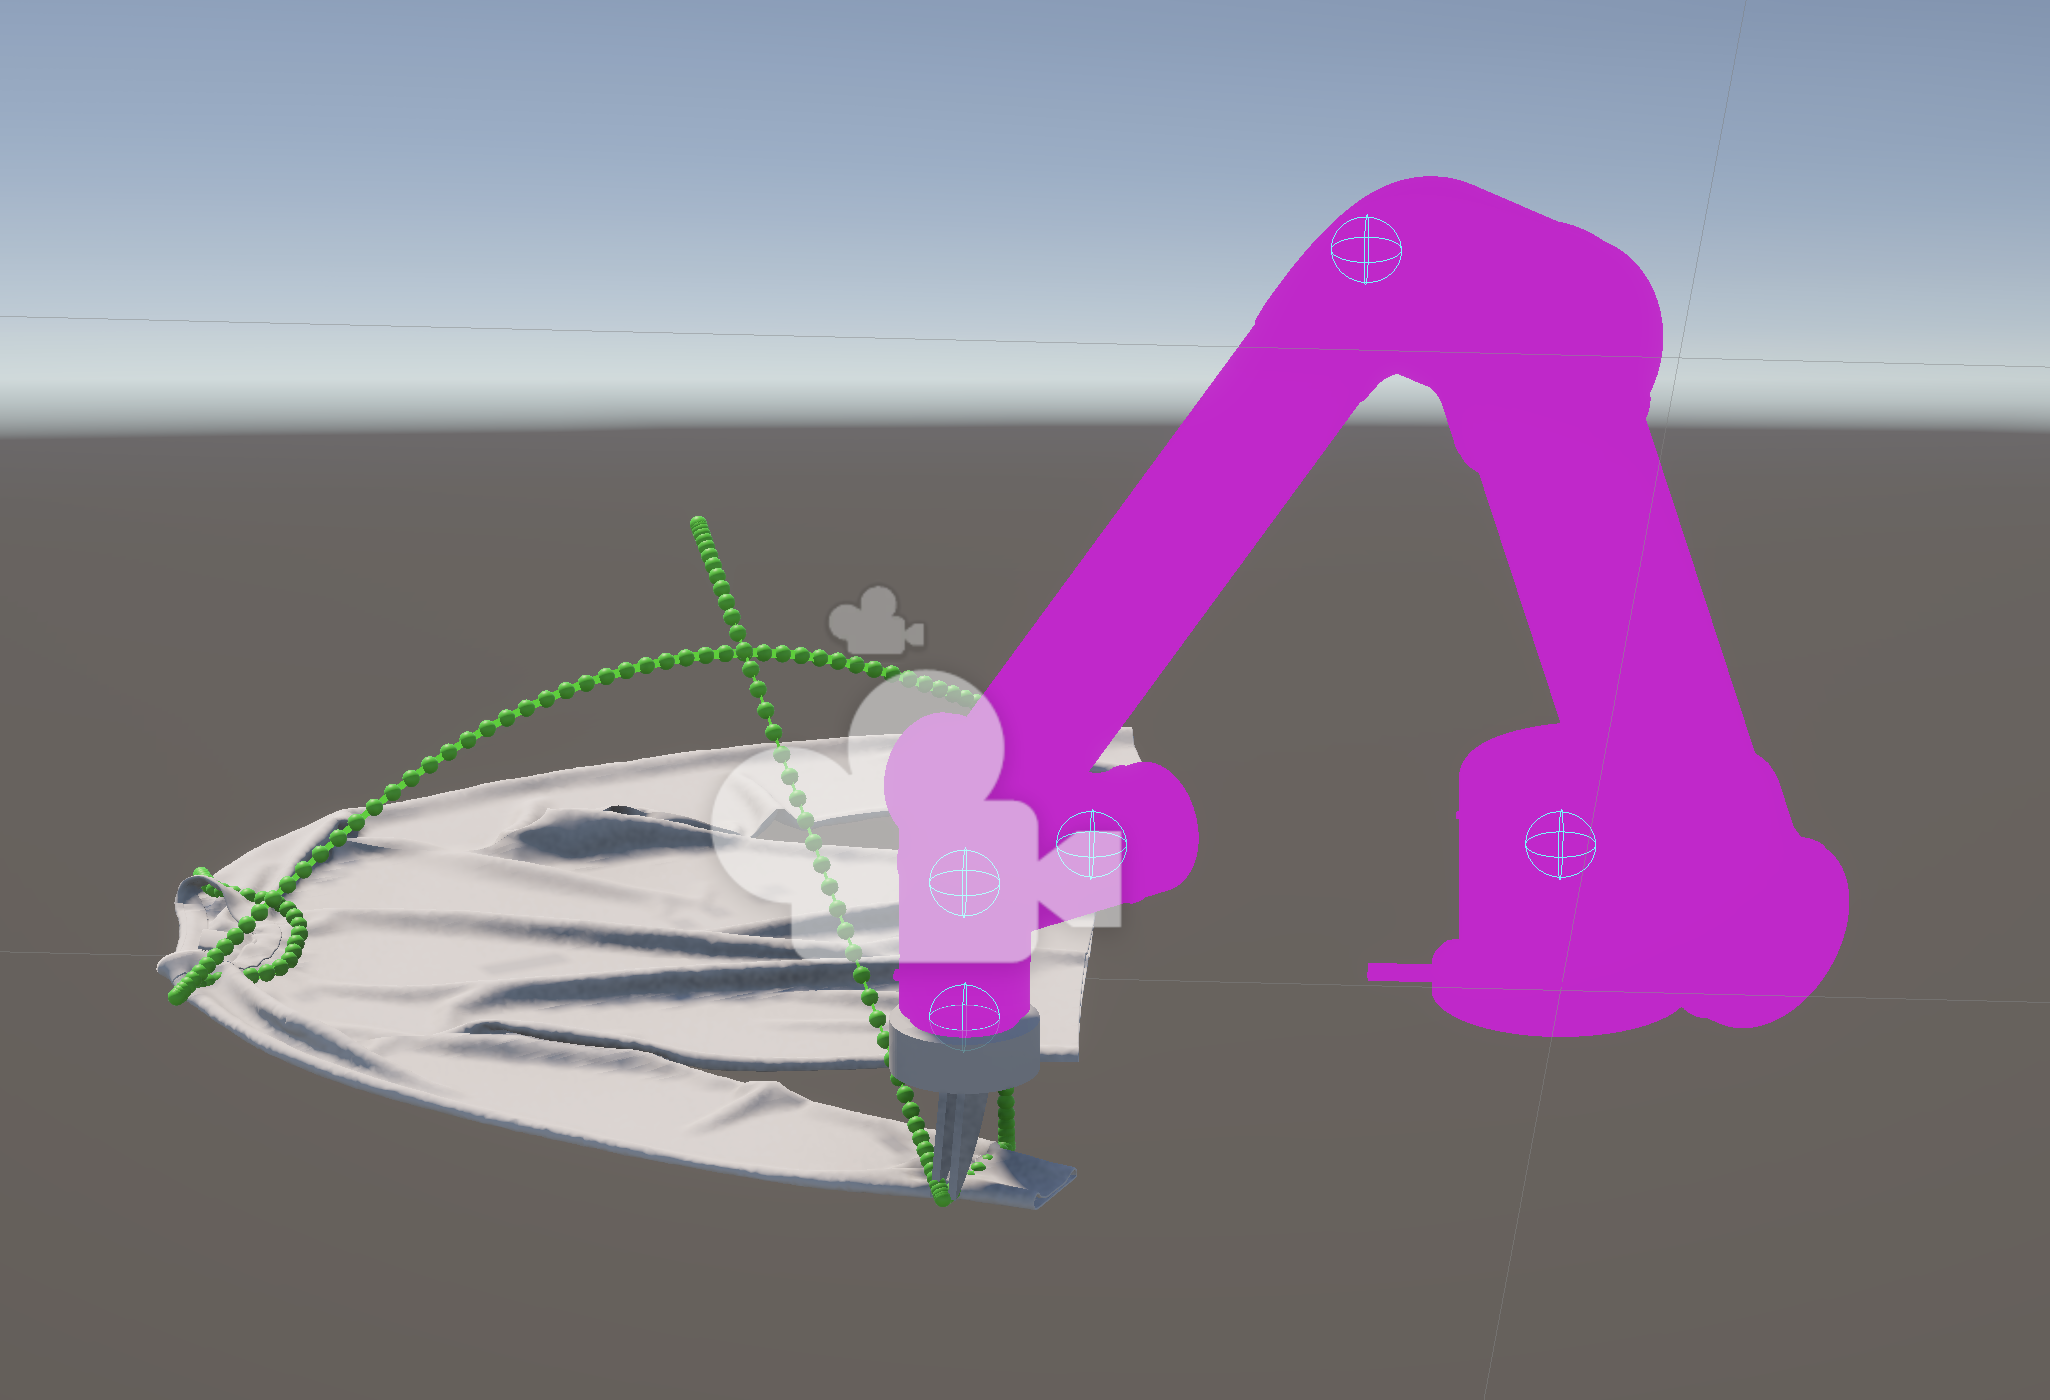
\includegraphics[width=0.75\linewidth]{figures/unity/polsino_sx.png}
    \caption{Visualizzazione traiettoria}
    \label{fig:polsino sx}
\end{figure}

La procedura viene ripetuta a ogni ciclo, aggiornando il comando sulla base dello stato corrente del robot. In questo modo, la pianificazione della traiettoria viene combinata con un controllo in retroazione che mira a ridurre gli errori di inseguimento e a migliorare la precisione del movimento.
Parallelamente all'esecuzione del moto, il nodo pubblica anche l'intera traiettoria pianificata su un topic dedicato. In Unity tale traiettoria viene rappresentata graficamente mediante una sequenza di sfere distribuite lungo il percorso, consentendo una verifica immediata della correttezza della pianificazione e del movimento dell'end-effector rispetto al maglione.

\begin{figure}[H]
    \centering
    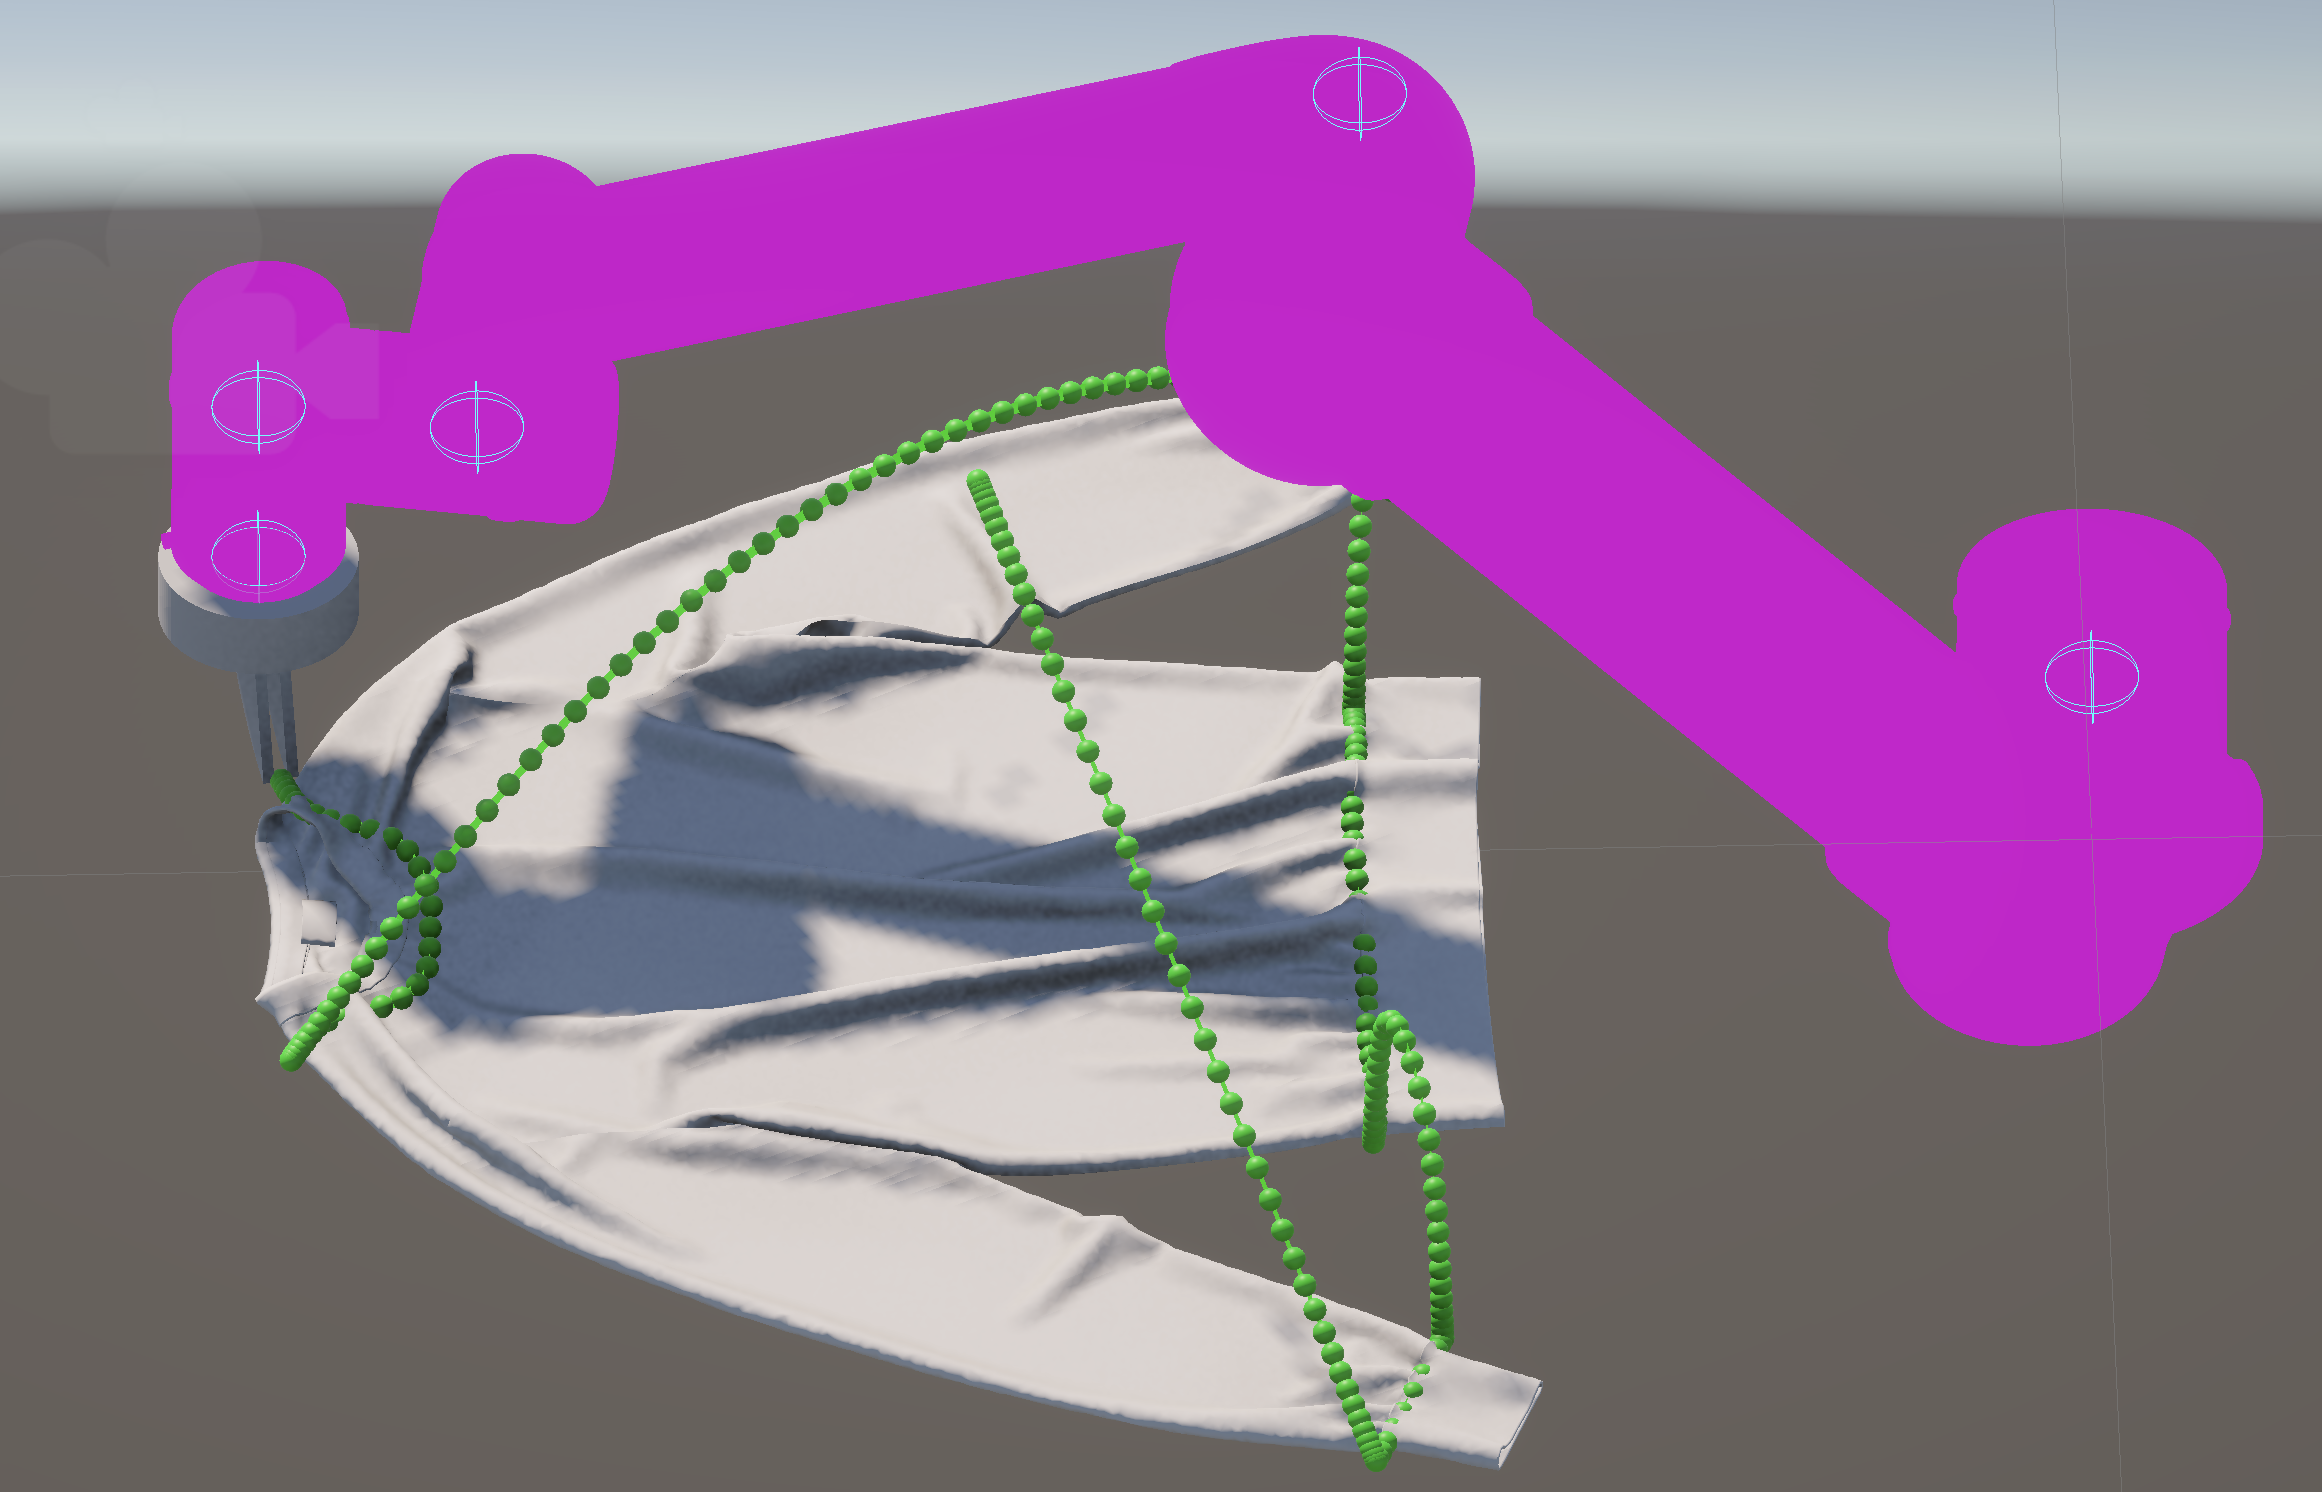
\includegraphics[width=0.75\linewidth]{figures/unity/fine_traiettoria.png}
    \caption{Fine traiettoria}
    \label{fig:fine traiettoria}
\end{figure}

\chapter{Utilizzo del robot reale UR5}
\label{chap:ur5_reale}

Dopo aver sviluppato e testato il sistema di controllo del robot in ambiente simulato con Unity, l'implementazione è stata estesa per consentire l'utilizzo del robot reale UR5.
Questa sezione descrive le modifiche apportate all'architettura e al flusso di lavoro per adattarsi alle specifiche del robot reale, garantendo un'integrazione efficace con il sistema di controllo basato su ROS~2.

\section{Polyscope e test preliminari}
Prima ancora di passare al robot reale, abbiamo fatto utilizzo di un ulteriore simulatore, ovvero Polyscope, che ci ha permesso di testare il sistema di controllo effettivo in un ambiente virtuale più vicino alla realtà, simulando il comportamento del robot UR5 e verificando la correttezza delle traiettorie pianificate e dei comandi inviati al robot.
Su Polyscope abbiamo utilizzato il driver UR5 ROS2 di default, ma un differente controller, ovvero il \texttt{forward\_position\_controller}, che ci ha permesso di utilizzare lo stesso metodo precedente per la trasmissione della traiettoria pianificata, ovvero la pubblicazione dei riferimenti punto per punto ad una certa frequenza.

\section{Test sul robot reale}
Dopo il processo precedente, il sistema è stato testato sul robot reale e le traiettorie pianificate sono state eseguite con successo, dimostrando l'efficacia del sistema di controllo sviluppato sebbene il metodo di pubblicazione dei riferimenti punto per punto ad una certa frequenza, anche elevata, non sia stata ottimale e presentava dei leggeri scatti durante l'esecuzione della traiettoria.
Motivo per il quale, è stato deciso di passare ad un differente controller ros2 che è quello di default del driver UR5, ovvero lo \texttt{scaled\_joint} e che utilizza un \textit{action server} e un \textit{action client} per la trasmissione della traiettoria pianificata, permettendo di inviare l'intera traiettoria in un'unica richiesta e ricevere una conferma di completamento al termine dell'esecuzione.

\subsection{Scelta del controller: \texttt{scaled\_joint\_trajectory\_controller}}

Il driver ROS~2 del robot UR mette a disposizione diversi controller. I due più rilevanti per questo lavoro sono il \texttt{forward\_position\_controller} e lo \texttt{scaled\_joint\_trajectory\_controller}.

Il \texttt{forward\_position\_controller} è un controller di tipo \emph{forward command}: riceve su un topic un vettore di posizioni articolari e lo inoltra direttamente all'interfaccia hardware.
Non esegue alcuna interpolazione, non applica limiti di velocità o accelerazione e non verifica il raggiungimento dell'obiettivo.
Il profilo di moto dipende interamente dal nodo che pubblica i comandi, che deve quindi inviare un nuovo setpoint a frequenza costante e senza interruzioni.
Un ritardo o un salto tra due setpoint successivi si traduce in un movimento brusco del robot.

Lo \texttt{scaled\_joint\_trajectory\_controller} è invece un controller di traiettoria: riceve, tramite l'action \texttt{FollowJointTrajectory},
una sequenza di punti (posizioni, velocità e istanti temporali) e si occupa di interpolarli e di eseguirli. Il termine \emph{scaled} indica che il tempo della traiettoria viene scalato in base al fattore di velocità
impostato sul teach pendant del robot: se l'operatore riduce la velocità o interviene una sospensione di sicurezza, la traiettoria rallenta
mantenendo la propria forma, senza accumulare errore di inseguimento.

\begin{table}[h]
\centering
\begin{tabular}{p{4cm}p{4.5cm}p{4.5cm}}
\toprule
 & \texttt{forward\_position} & \texttt{scaled\_joint\_trajectory} \\
\midrule
Ingresso & singolo setpoint (topic) & traiettoria completa (action) \\
Interpolazione & assente & presente \\
Temporizzazione & a carico del nodo & gestita dal controller \\
Tolleranze e esito & assenti & presenti (feedback e risultato) \\
Annullamento & non previsto & previsto (cancellazione del goal) \\
Scalatura di velocità & no & sì (teach pendant) \\
\bottomrule
\end{tabular}
\caption{Confronto tra i due controller.}
\end{table}

Si è scelto lo \texttt{scaled\_joint\_trajectory\_controller} per tre motivi.
In primo luogo, la traiettoria viene completamente calcolata \emph{offline}
a partire dalla traiettoria cartesiana e inviata come un unico goal: il controller
garantisce la temporizzazione, mentre con il \texttt{forward\_position\_controller}
la regolarità del moto dipenderebbe dalla periodicità di un nodo Python
non real-time. In secondo luogo, il controller fornisce feedback, verifica
delle tolleranze e possibilità di annullare il movimento, utili per
controllare l'esecuzione e fermare il robot in caso di anomalie. Infine, la
scalatura del tempo rispetta i limiti e gli arresti di sicurezza imposti
dal pendant, aspetto rilevante in un'applicazione in cui il robot opera
in prossimità dell'operatore. Infine, grazie all'interpolazione interna, il controller garantisce un movimento più fluido e privo di scatti, migliorando la qualità complessiva dell'esecuzione della traiettoria pianificata.

\chapter{Pianificazione della traiettoria cartesiana}
\label{chap:pianificazione_traiettoria}

La pianificazione della traiettoria ha lo scopo di definire il movimento dell'organo terminale del robot nello spazio cartesiano, a partire da un insieme di punti tridimensionali già individuati sulla maglia. Questi punti rappresentano i riferimenti geometrici che il robot deve seguire durante le operazioni di cucitura simulata lungo i polsini, il fondo della maglia e il colletto.

Dal punto di vista fisico, non è sufficiente collegare direttamente i punti mediante segmenti rettilinei. Una successione di segmenti può infatti introdurre discontinuità nella direzione del movimento e richiedere variazioni istantanee della velocità in corrispondenza dei vertici. Tali condizioni non sono compatibili con un movimento regolare, poiché comporterebbero accelerazioni elevate e sollecitazioni dinamiche non desiderabili.

La traiettoria viene quindi costruita attraverso tre operazioni principali:
\begin{enumerate}
    \item organizzazione dei punti in segmenti distinti, comprendenti le cuciture e i raccordi di collegamento;
    \item interpolazione geometrica mediante spline cubiche, per ottenere percorsi continui;
    \item assegnazione di una legge temporale al movimento, attraverso profili di velocità e accelerazione limitati.
\end{enumerate}

Il risultato è una traiettoria cartesiana descritta, per ogni istante, dalla posizione desiderata dell'organo terminale, dalla sua velocità lineare e dal suo orientamento.
Grazie alla sua versatilità, il metodo realizzato può essere applicato sia al caso simulato con Unity che al caso reale con il robot UR5, con la possibilità di adattare i parametri cinematici in funzione delle esigenze operative.

\section{Organizzazione geometrica del percorso}

La funzione \texttt{genera\_traiettoria\_diversa()} organizza il percorso in otto segmenti consecutivi. Tale suddivisione permette di distinguere le operazioni di cucitura vere e proprie dai movimenti necessari per passare da una regione della maglia alla successiva.

Indicando con $\mathbf{P}_{\mathrm{start}}$ la posizione iniziale dell'organo terminale e con $\mathcal{P}_{\mathrm{sx}}$, $\mathcal{P}_{\mathrm{fondo}}$, $\mathcal{P}_{\mathrm{dx}}$ e $\mathcal{P}_{\mathrm{coll}}$ gli insiemi di punti relativi, rispettivamente, al polsino sinistro, al fondo, al polsino destro e al colletto, la sequenza è organizzata come segue:

\begin{enumerate}
    \item avvicinamento dalla posizione iniziale al primo punto del polsino sinistro;
    \item percorrenza dei punti del polsino sinistro;
    \item raccordo dal polsino sinistro al fondo maglia;
    \item percorrenza dei punti del fondo maglia;
    \item raccordo dal fondo maglia al polsino destro;
    \item percorrenza dei punti del polsino destro;
    \item raccordo dal polsino destro al colletto;
    \item percorrenza dei punti del colletto.
\end{enumerate}

Questa suddivisione consente di assegnare a ciascun tratto parametri di movimento differenti, in funzione della sua natura geometrica e delle esigenze operative.

\subsection{Interpolazione dei punti dei polsini}

Per i polsini sono inizialmente disponibili due punti estremi, che identificano l'inizio e la fine del tratto da percorrere. Per aumentare la densità dei riferimenti geometrici, vengono inseriti due punti intermedi mediante interpolazione lineare.

Indicando con $\mathbf{P}_0$ e $\mathbf{P}_1$ gli estremi del segmento, i punti intermedi sono definiti da

\begin{equation}
    \mathbf{P}_{1/3}
    = \mathbf{P}_0 + \frac{1}{3}
    \left(\mathbf{P}_1-\mathbf{P}_0\right),
\end{equation}

\begin{equation}
    \mathbf{P}_{2/3}
    = \mathbf{P}_0 + \frac{2}{3}
    \left(\mathbf{P}_1-\mathbf{P}_0\right).
\end{equation}

Si ottiene così una sequenza di quattro punti complessivi. L'inserimento di punti intermedi non modifica la geometria del segmento rettilineo iniziale, ma fornisce più riferimenti per la successiva interpolazione.

\subsection{Uniformazione della quota dei punti - Caso UR5 simulato}

Per la gestione delle coordinate lungo l'asse \textit{z} viene utilizzata distanza fissa, corrispondente a quella tra la telecamera e il maglione, precedentemente misurata attraverso script.

\subsection{Uniformazione della quota dei punti - Caso UR5 reale}

Per ridurre le variazioni di quota tra i diversi riferimenti della maglia, la coordinata verticale dei punti dei polsini e del colletto viene uniformata utilizzando una quota di riferimento calcolata a partire dai punti del fondo.

Indicando con $z_i$ la coordinata verticale dell'$i$-esimo punto del fondo, la quota comune è

\begin{equation}
    z_{\mathrm{ref}}
    = \frac{1}{N_f}\sum_{i=1}^{N_f} z_i,
    \label{eq:quota_riferimento}
\end{equation}

dove $N_f$ è il numero di punti utilizzati per descrivere il fondo.

Per i punti appartenenti ai polsini e al colletto, la coordinata verticale viene quindi sostituita con

\begin{equation}
    z_i' = z_{\mathrm{ref}}.
\end{equation}

In questo modo, i punti di tali regioni risultano complanari rispetto alla quota scelta, mentre i punti del fondo conservano le proprie coordinate. La scelta semplifica la geometria del percorso e riduce le variazioni verticali introdotte dai punti di riferimento.

È importante precisare che questa operazione costituisce un'approssimazione geometrica: non descrive direttamente la deformazione della maglia né garantisce che la sua superficie reale sia perfettamente piana.

\section{Costruzione dei raccordi tra i segmenti}

I segmenti di cucitura sono collegati mediante tratti di transizione. Lo scopo dei raccordi è evitare che il robot debba passare direttamente da una regione della maglia a un'altra seguendo un percorso che attraversi inutilmente la superficie intermedia.

La funzione \texttt{build\_trapezoids()} costruisce questi raccordi sulla base della distanza tra l'estremo del segmento precedente e l'inizio di quello successivo.

Siano $\mathbf{P}_a$ il punto finale del segmento precedente e $\mathbf{P}_b$ il punto iniziale del segmento successivo. La distanza tra i due punti, proiettati sul piano orizzontale, è calcolata come

\begin{equation}
    d_{xy}
    = \sqrt{(x_b-x_a)^2+(y_b-y_a)^2}.
    \label{eq:distanza_xy}
\end{equation}

La geometria del raccordo dipende da tale distanza:

\begin{itemize}
    \item se $d_{xy} \geq 0.1\,\mathrm{m}$, vengono introdotti due punti intermedi;
    \item se $0.03\,\mathrm{m} \leq d_{xy} < 0.1\,\mathrm{m}$, viene introdotto un solo punto intermedio;
    \item se $d_{xy} < 0.03\,\mathrm{m}$, non vengono aggiunti punti intermedi.
\end{itemize}

Nel caso di due punti intermedi, le loro coordinate orizzontali sono ottenute dividendo lo spostamento in tre parti uguali:

\begin{equation}
    \mathbf{p}_{1,xy}
    = \mathbf{p}_{a,xy}
    + \frac{1}{3}
    \left(\mathbf{p}_{b,xy}-\mathbf{p}_{a,xy}\right),
\end{equation}

\begin{equation}
    \mathbf{p}_{2,xy}
    = \mathbf{p}_{a,xy}
    + \frac{2}{3}
    \left(\mathbf{p}_{b,xy}-\mathbf{p}_{a,xy}\right).
\end{equation}

La quota dei punti intermedi viene aumentata di una quantità prefissata:

\begin{equation}
    z_{\mathrm{up}} = z_a + h,
    \qquad h=0.1\,\mathrm{m}.
    \label{eq:quota_raccordo}
\end{equation}

Quando viene inserito un solo punto intermedio, le sue coordinate orizzontali corrispondono al punto medio tra gli estremi. La quota viene calcolata con la stessa regola.

Dal punto di vista fisico, il sollevamento introduce un percorso che si allontana dalla superficie della maglia durante il trasferimento tra due regioni distanti. Questo accorgimento può ridurre il rischio di interferenza con il tessuto durante gli spostamenti, ma non costituisce una garanzia di assenza di collisioni: tale proprietà dipende anche dalla geometria effettiva della maglia, dalla posizione del tessuto e dalle dimensioni dell'organo terminale.

I raccordi vengono pertanto considerati come segmenti autonomi, ai quali è possibile assegnare limiti cinematici differenti da quelli dei tratti di cucitura.

\section{Interpolazione mediante spline cubiche}

Una volta definiti i punti di ciascun segmento, è necessario costruire una curva continua che li attraversi. A questo scopo vengono utilizzate spline cubiche naturali, calcolate separatamente per le tre coordinate cartesiane.

Sia un segmento descritto da $M$ punti tridimensionali

\begin{equation}
    \mathbf{P}_i =
    \begin{bmatrix}
        x_i & y_i & z_i
    \end{bmatrix}^{T},
    \qquad i=0,\ldots,M-1.
\end{equation}

Per associare ai punti un parametro adimensionale crescente lungo il percorso, viene calcolata la lunghezza cumulativa della poligonale:

\begin{equation}
    \ell_0 = 0,
\end{equation}

\begin{equation}
    \ell_i = \ell_{i-1}
    + \left\|\mathbf{P}_i-\mathbf{P}_{i-1}\right\|,
    \qquad i=1,\ldots,M-1.
\end{equation}

Il parametro viene poi normalizzato rispetto alla lunghezza totale della poligonale:

\begin{equation}
    u_i = \frac{\ell_i}{\ell_{M-1}},
    \qquad u_i \in [0,1].
    \label{eq:parametro_spline}
\end{equation}

La normalizzazione permette di descrivere ciascun segmento mediante un parametro che varia da zero a uno, indipendentemente dalla sua lunghezza fisica.

Vengono quindi costruite tre funzioni spline distinte:

\begin{equation}
    x=x(u), \qquad y=y(u), \qquad z=z(u).
\end{equation}

La curva cartesiana risultante è

\begin{equation}
    \mathbf{r}(u)=
    \begin{bmatrix}
        x(u)\\
        y(u)\\
        z(u)
    \end{bmatrix}.
    \label{eq:curva_cartesiana}
\end{equation}

Ogni coordinata è interpolata mediante una funzione polinomiale cubica definita a tratti. Le spline naturali impongono che la derivata seconda sia nulla agli estremi del segmento:

\begin{equation}
    x''(0)=x''(1)=0,
\end{equation}

con condizioni analoghe per $y(u)$ e $z(u)$.

La costruzione garantisce la continuità della posizione e della derivata prima all'interno del singolo segmento, evitando gli spigoli tipici della connessione diretta tra segmenti rettilinei. La derivata seconda è inoltre continua nei nodi interni della spline.

È tuttavia necessario distinguere la regolarità dei singoli segmenti dalla regolarità dell'intera traiettoria: poiché ogni tratto viene interpolato separatamente, la continuità delle derivate tra segmenti consecutivi non è automaticamente garantita dalla sola interpolazione cubica. I raccordi geometrici e le successive leggi temporali contribuiscono a rendere il movimento più regolare, ma la continuità globale deve essere valutata sui risultati ottenuti.

\section{Lunghezza della curva e parametro di avanzamento}

Il parametro $u$ descrive la geometria della spline, ma non rappresenta direttamente la distanza percorsa. Infatti, incrementi uguali di $u$ non corrispondono necessariamente a incrementi uguali di lunghezza lungo una curva.

Per associare al percorso una coordinata spaziale fisica, si considera la lunghezza d'arco. La lunghezza totale della spline è definita da

\begin{equation}
    L = \int_0^1
    \left\|\frac{d\mathbf{r}(u)}{du}\right\|du.
    \label{eq:lunghezza_arco}
\end{equation}

Nel codice, tale integrale viene approssimato numericamente campionando la curva in un elevato numero di punti e sommando le distanze euclidee tra campioni consecutivi:

\begin{equation}
    L \simeq
    \sum_{i=1}^{N_s-1}
    \left\|\mathbf{r}(u_i)-\mathbf{r}(u_{i-1})\right\|,
\end{equation}

dove $N_s$ è il numero di campioni impiegati per l'approssimazione.

Questa grandezza, espressa in metri, rappresenta la distanza effettiva lungo la curva interpolata e costituisce il riferimento per la pianificazione della velocità.

Introducendo una coordinata di avanzamento $s(t)$, con

\begin{equation}
    0 \leq s(t) \leq L,
\end{equation}

la posizione cartesiana nel tempo può essere espressa come

\begin{equation}
    \mathbf{x}(t)=\mathbf{r}\left(u(t)\right),
\end{equation}

dove $u(t)$ è ricavato dal rapporto tra l'avanzamento lungo la curva e la lunghezza totale, mediante la relazione $u(t)=s(t)/L$.

In questo modo vengono separati due problemi distinti: la definizione della forma geometrica del percorso e la definizione della velocità con cui tale percorso viene attraversato.

\section{Pianificazione della velocità e dell'accelerazione}

La sola definizione della curva non determina quanto rapidamente il robot debba percorrerla. Per descrivere il movimento nel tempo viene quindi associato a ciascun segmento un profilo di velocità trapezoidale, o triangolare quando non è disponibile spazio sufficiente per raggiungere il valore massimo di velocità.

Il profilo è definito attraverso due parametri principali:
\begin{itemize}
    \item $v_{\max}$, velocità lineare massima lungo la curva;
    \item $a_{\max}$, modulo massimo dell'accelerazione tangenziale.
\end{itemize}

La velocità scalare lungo il percorso è indicata con

\begin{equation}
    v(t)=\frac{ds(t)}{dt}.
\end{equation}

L'accelerazione tangenziale è invece

\begin{equation}
    a_t(t)=\frac{dv(t)}{dt}.
\end{equation}

Nel caso di un profilo trapezoidale, il moto è suddiviso in tre fasi:
\begin{enumerate}
    \item accelerazione, durante la quale la velocità cresce da zero fino al valore massimo;
    \item regime, durante il quale la velocità rimane costante;
    \item decelerazione, durante la quale la velocità diminuisce fino a zero.
\end{enumerate}

Assumendo accelerazione costante durante la prima fase, la velocità cresce secondo

\begin{equation}
    v(t)=a_{\max}t,
\end{equation}

mentre lo spazio percorso è

\begin{equation}
    s(t)=\frac{1}{2}a_{\max}t^2.
\end{equation}

Il tempo necessario a raggiungere la velocità massima è

\begin{equation}
    t_a=\frac{v_{\max}}{a_{\max}},
\end{equation}

e la distanza percorsa durante l'accelerazione è

\begin{equation}
    s_a=\frac{v_{\max}^2}{2a_{\max}}.
\end{equation}

Una fase di decelerazione simmetrica richiede una distanza analoga. Se la lunghezza disponibile non è sufficiente a contenere entrambe le fasi e un tratto a velocità costante, il profilo diventa triangolare: la velocità massima nominale non viene raggiunta.

La funzione di pianificazione genera un profilo spaziale di velocità lungo la curva e lo converte successivamente in una successione di istanti temporali. Il tempo viene ottenuto integrando numericamente la relazione

\begin{equation}
    dt=\frac{ds}{v(s)}.
\end{equation}

Per campioni consecutivi, l'incremento temporale viene approssimato utilizzando la velocità media:

\begin{equation}
    \Delta t_i \simeq
    \frac{s_i-s_{i-1}}
    {\left(v_i+v_{i-1}\right)/2},
    \label{eq:incremento_temporale}
\end{equation}

quando la velocità media è sufficientemente diversa da zero.

Il tempo cumulativo è quindi

\begin{equation}
    t_i=\sum_{j=1}^{i}\Delta t_j.
\end{equation}

La relazione tra tempo e avanzamento viene poi interpolata per ottenere campioni temporali uniformi. Questo passaggio consente di descrivere la traiettoria attraverso una sequenza ordinata di posizioni e velocità.

\subsection{Parametri cinematici dei segmenti}

Nel codice vengono utilizzati limiti differenti in funzione del tipo di tratto. Per i segmenti ordinari di cucitura e per i raccordi non trattati come casi speciali, i valori di riferimento sono

\begin{equation}
    v_{\max}=0.06\,\mathrm{m/s},
    \qquad
    a_{\max}=0.005\,\mathrm{m/s^2}.
\end{equation}

Per il segmento finale relativo al colletto vengono utilizzati valori inferiori:

\begin{equation}
    v_{\max}=0.03\,\mathrm{m/s},
    \qquad
    a_{\max}=0.002\,\mathrm{m/s^2}.
\end{equation}

Per il primo segmento di avvicinamento e per il raccordo identificato dal codice con indice sei vengono invece assegnati valori più elevati:

\begin{equation}
    v_{\max}=0.2\,\mathrm{m/s},
    \qquad
    a_{\max}=0.06\,\mathrm{m/s^2}.
\end{equation}

La riduzione dei limiti cinematici sul colletto è coerente con la scelta di percorrere più lentamente un tratto che richiede maggiore attenzione geometrica. Si tratta, tuttavia, di una scelta progettuale e non di un limite fisico universale: i valori devono essere verificati sperimentalmente rispetto alla precisione richiesta, alla risposta del robot e all'interazione con il tessuto.

\section{Calcolo della velocità cartesiana}

Una volta definita la legge temporale, è possibile determinare la velocità cartesiana desiderata dell'organo terminale.

Dalla relazione

\begin{equation}
    \mathbf{x}(t)=\mathbf{r}(u(t)),
\end{equation}

applicando la regola della derivazione composta si ottiene

\begin{equation}
    \dot{\mathbf{x}}(t)
    =\frac{d\mathbf{r}}{du}\frac{du}{dt}.
    \label{eq:velocita_catena}
\end{equation}

La velocità cartesiana è diretta lungo la tangente alla curva. Per imporre che il suo modulo coincida con la velocità scalare pianificata $v(t)$, viene utilizzato il versore tangente

\begin{equation}
    \mathbf{t}(u)=
    \frac{\mathbf{r}'(u)}
    {\|\mathbf{r}'(u)\|}.
\end{equation}

La velocità desiderata può quindi essere scritta come

\begin{equation}
    \dot{\mathbf{x}}_d(t)
    =v(t)\mathbf{t}(u(t)).
    \label{eq:velocita_cartesiana}
\end{equation}

Esplicitando le componenti, si ottiene

\begin{equation}
    v_x(t)=
    v(t)\frac{x'(u)}{\|\mathbf{r}'(u)\|},
\end{equation}

\begin{equation}
    v_y(t)=
    v(t)\frac{y'(u)}{\|\mathbf{r}'(u)\|},
\end{equation}

\begin{equation}
    v_z(t)=
    v(t)\frac{z'(u)}{\|\mathbf{r}'(u)\|}.
\end{equation}

Questa formulazione è importante dal punto di vista fisico perché separa il modulo della velocità dalla direzione del movimento. Il profilo temporale stabilisce quanto rapidamente avanzare, mentre la derivata della spline determina in quale direzione muoversi.

La norma della velocità cartesiana risulta idealmente pari a $v(t)$:

\begin{equation}
    \|\dot{\mathbf{x}}_d(t)\|=v(t),
\end{equation}

purché la derivata della curva non sia nulla.

\section{Pianificazione dell'orientamento dell'organo terminale}

Oltre alla posizione, è necessario definire l'orientamento dell'organo terminale durante il movimento. Tale orientamento determina la direzione degli assi locali dell'utensile e contribuisce a stabilire come esso si presenta rispetto alla superficie della maglia.

Per i segmenti senza un orientamento imposto, il codice costruisce una terna cartesiana a partire dalla direzione tangente al percorso. Per ogni punto campionato, la direzione tangente viene utilizzata come asse locale $x_e$:

\begin{equation}
    \mathbf{x}_e=
    \frac{\mathbf{r}'(u)}
    {\|\mathbf{r}'(u)\|}.
\end{equation}

Viene quindi introdotto un vettore di riferimento verticale

\begin{equation}
    \mathbf{z}_{\mathrm{ref}}=
    \begin{bmatrix}
        0 & 0 & -1
    \end{bmatrix}^{T}.
\end{equation}

Il secondo asse della terna viene calcolato mediante il prodotto vettoriale:

\begin{equation}
    \mathbf{y}_e=
    \frac{\mathbf{z}_{\mathrm{ref}}\times\mathbf{x}_e}
    {\|\mathbf{z}_{\mathrm{ref}}\times\mathbf{x}_e\|}.
\end{equation}

Il terzo asse viene infine ricostruito per ottenere una terna ortogonale:

\begin{equation}
    \mathbf{z}_e=\mathbf{x}_e\times\mathbf{y}_e.
\end{equation}

La matrice di orientamento desiderata è quindi

\begin{equation}
    R_d=
    \begin{bmatrix}
        \mathbf{x}_e & \mathbf{y}_e & \mathbf{z}_e
    \end{bmatrix}.
    \label{eq:matrice_orientamento}
\end{equation}

Dal punto di vista geometrico, questa costruzione allinea il primo asse locale alla direzione di avanzamento e utilizza la verticale come riferimento per definire gli altri due assi. In questo modo l'orientamento varia in relazione alla forma della curva, anziché essere mantenuto arbitrariamente costante.

Quando il prodotto vettoriale impiegato per calcolare $\mathbf{y}_e$ ha norma molto piccola, la direzione tangente è quasi parallela al vettore verticale di riferimento. In tale condizione la costruzione diventa numericamente mal condizionata; il codice prevede un vettore alternativo per evitare una divisione per una norma prossima a zero.

\subsection{Transizioni tra orientamenti}

Nei raccordi tra segmenti, l'orientamento iniziale e quello finale possono essere differenti. Per evitare una variazione improvvisa della posa, viene utilizzata l'interpolazione sferica dei quaternioni, nota come SLERP (\textit{Spherical Linear Interpolation}).

Indicando con $R_0$ e $R_1$ le matrici di orientamento agli estremi del raccordo, si convertono tali orientamenti in rappresentazioni quaternioniche e si interpola tra le due pose in funzione del parametro normalizzato $u$:

\begin{equation}
    R_d(u)=\operatorname{SLERP}(R_0,R_1,u).
\end{equation}

La SLERP segue un percorso regolare nello spazio delle rotazioni e consente di evitare l'interpolazione indipendente degli angoli di Eulero, che può produrre comportamenti poco regolari.

La transizione dell'orientamento viene quindi coordinata con l'avanzamento lungo il raccordo. La posizione segue la spline cartesiana, mentre l'orientamento evolve gradualmente tra le due configurazioni estreme.

\section{Concatenazione della traiettoria completa}

Ogni segmento produce una sequenza temporale di posizioni, velocità cartesiane e orientamenti. Al termine della pianificazione, le sequenze vengono concatenate mantenendo l'ordine dei tratti definito in precedenza.

La traiettoria risultante può essere rappresentata come

\begin{equation}
    \mathcal{T}=
    \left\{
    \mathbf{x}_d(t_i),
    \dot{\mathbf{x}}_d(t_i),
    R_d(t_i)
    \right\}_{i=0}^{N-1},
\end{equation}

dove $N$ è il numero totale di campioni.

Per ogni istante campionato sono quindi disponibili:
\begin{itemize}
    \item la posizione cartesiana desiderata $\mathbf{x}_d(t_i)$;
    \item la velocità lineare desiderata $\dot{\mathbf{x}}_d(t_i)$;
    \item l'orientamento desiderato $R_d(t_i)$.
\end{itemize}

La pianificazione produce così una descrizione cinematica completa del movimento nello spazio cartesiano. La traiettoria non specifica soltanto quali punti attraversare, ma anche come procedere lungo il percorso e come orientare l'organo terminale durante ciascun tratto.

\section{Considerazioni fisiche e limiti del modello}

La metodologia adottata consente di controllare separatamente la geometria del percorso e la sua evoluzione temporale. L'interpolazione con spline cubiche riduce le discontinuità geometriche all'interno dei singoli segmenti, mentre i profili di velocità e accelerazione limitano la rapidità con cui il percorso viene attraversato.

Questi aspetti sono particolarmente rilevanti nel contesto della manipolazione di un tessuto. Un movimento troppo rapido o caratterizzato da variazioni brusche può aumentare le sollecitazioni dinamiche e compromettere la precisione con cui l'utensile segue la linea desiderata. Al contrario, una velocità più contenuta nei tratti delicati permette di adottare una strategia di movimento più prudente.

È tuttavia importante distinguere la pianificazione cinematica dalla modellazione dinamica dell'interazione con il tessuto. Il profilo di velocità limita la velocità tangenziale e l'accelerazione lungo il percorso, ma non calcola direttamente le forze di contatto, la tensione della maglia o la sua deformazione. Inoltre, l'accelerazione cartesiana totale non coincide necessariamente con la sola accelerazione tangenziale, poiché la curvatura del percorso introduce anche una componente normale:

\begin{equation}
    \mathbf{a}(t)=
    a_t(t)\mathbf{t}(t)
    +v(t)^2\kappa(t)\mathbf{n}(t),
\end{equation}

dove $\kappa(t)$ è la curvatura locale e $\mathbf{n}(t)$ è il versore normale alla traiettoria. Di conseguenza, anche quando il modulo dell'accelerazione tangenziale è limitato, curve molto strette possono generare accelerazioni normali significative.

Infine, la pianificazione viene eseguita separatamente per ciascun segmento. La continuità della posizione tra i tratti è favorita dalla costruzione dei punti di raccordo, ma la continuità della velocità e dell'accelerazione ai confini tra segmenti dipende anche dai profili temporali assegnati e dalla loro concatenazione. Per questo motivo, la verifica della traiettoria completa mediante grafici di posizione, velocità e orientamento costituisce un passaggio importante per individuare eventuali variazioni indesiderate.

In sintesi, il metodo consente di ottenere un percorso cartesiano regolare e parametrizzato nel tempo, con una velocità adattata alle diverse fasi del movimento. La qualità fisica del movimento dipende tuttavia anche dalla curvatura locale, dalla continuità tra segmenti e dall'effettiva interazione tra organo terminale e tessuto.


\chapter{Pianificazione Traiettorie e Controllo}

\section{Pianificazione}
Traiettorie generate con MoveIt! da punti segmentati. Per polsini: ellisse fitting su contour. Velocità: 50 mm/s, accelerazione 500 mm/s². Filtraggio spline per smoothing.

\section{Controllo UR5}
Controllo ibrido: posizione cartesiana con servo (impedenza 1000 N/m). Feedback visivo ogni 10 cicli per compensare deformazioni (errore < 3 mm).

Pseudocodice:
\begin{verbatim}
while not trajectory_complete:
    current_pose = get_ur5_pose()
    target_pose = next_waypoint()
    delta = target_pose - current_pose
    cmd = PID(delta)
    ur5.move(cmd)
\end{verbatim}

\chapter{Risultati e Conclusioni}

Test su 20 maglioncini: successo 85\% (fallimenti per occlusioni). Tempi: segmentazione 20 ms, traiettoria 1.2 s.

Le sfide principali (deformabilità, illuminazione) sono state mitigate, dimostrando fattibilità. Futuri sviluppi: multi-view, RL per adattamento, integrazione force-torque.

\listoffigures

\bibliographystyle{plain}
\bibliography{references}



%----------------



% \newpage
% \chapter{Sistema}
% \textcolor{red}{NOTA valido per ogni capitolo: }inserire all'inizio di ogni capitolo una brevissima descrizione del contenuto del capitolo stesso.\\
% \newline
% \textcolor{red}{NOTA:} capitolo opzionale.
% Solo se necessario per comprendere quanto svolto, inserite un capitolo dedicato al sistema su cui avete lavorato (es drone quadrirotore, ballbot ..) dove descrivete ad esempio come è fatto il sistema, come si modella matematicamente e come si può controllare. Nel capitolo inserite solo le informazioni che avete effettivamente utilizzato per svolgere il task assegnatovi (\textcolor{red}{evitate il copia e incolla dalle vecchie relazioni}). Mettete la fonte da cui avete preso le informazioni (es vecchia relazione \cite{Relazione1}).
% \chapter{Modello matematico}
% \chapter{Controllo}

% \newpage
% \chapter{Hardware}
% \label{Hardware}
% Inserire sempre un capitolo "Hardware" dove si descrivono tutti i componenti hardware utilizzati (schede, sensori, attuatori..). Dedicare un paragrafo ad ogni componente. Per ogni componente riportare le seguenti informazioni: modello specifico, riferimento bibliografico con link ad un sito web con la documentazione del componente (es \cite{DCdriver}), immagine, pinout, solo le informazioni rilevanti per lo svolgimento del task.
% \chapter{Componente1}
% \chapter{Componente2}
% \chapter{Schema dei collegamenti}
% Inserire uno schema dei collegamenti analogo a quello in Figura \ref{fig:schema}. Si suggerisce per lo scopo di usare il software "draw.io". Nello schema riportare tutti i collegamenti tra i componenti, specificando quale pin di un componente1 si collega con quale pin di un componente2 (per la maggior parte dei collegamenti dovete cioè avere una linea con 2 label). \\
% Inserire anche una descrizione testuale dello schema.

% \begin{figure}[H]
% \centering
% 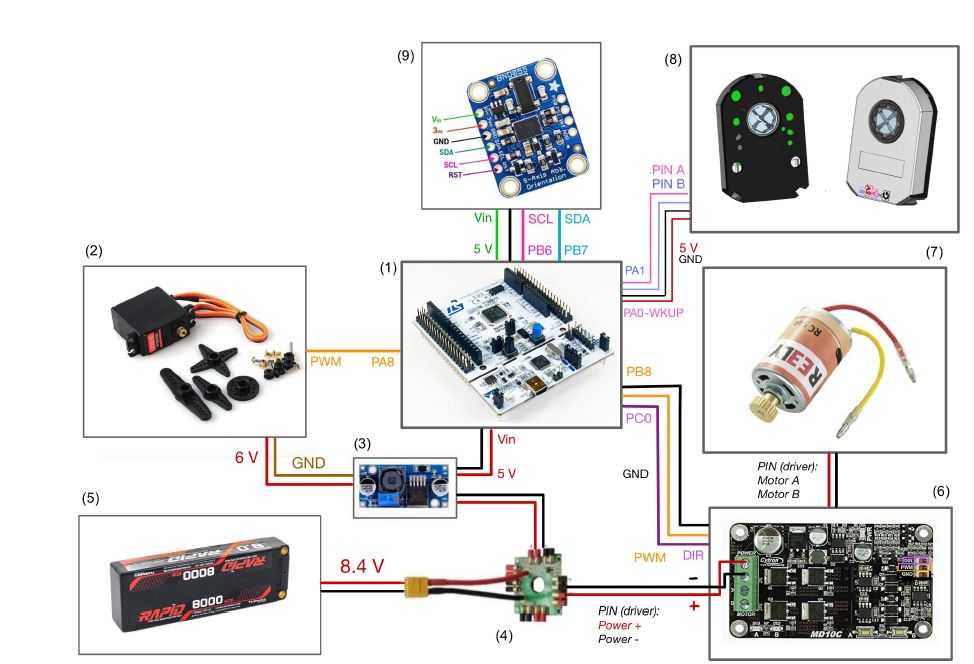
\includegraphics[width=0.8\textwidth,keepaspectratio]{figures/Schema.JPG}
% \caption{Schema dei collegamenti}
% \label{fig:schema}
% \end{figure}


% \chapter{Software}
% Nell'introduzione al capitolo specificate anche la versione dell'STM32CubeIDE e dell'STM32CubeMX che avete usato (se avete cambiato versione nel corso del progetto mettete l'ultima, quella su cui è sviluppato il codice che consegnate).

% \chapter{Diagramma di flusso}
% Inserire un diagramma di flusso analogo a quello in Figura \ref{fig:diagramma} che spiega il funzionamento generale del codice sviluppato. Inserire anche una descrizione testuale del funzionamento.

% \begin{figure}[H]
% \centering
% 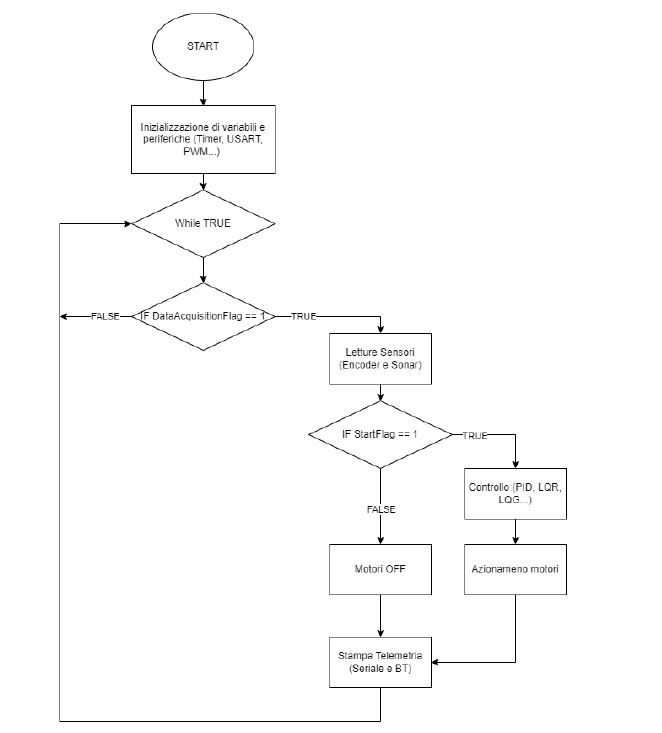
\includegraphics[width=0.8\textwidth,keepaspectratio]{figures/diagramma.JPG}
% \caption{Diagramma di flusso del codice sviluppato}
% \label{fig:diagramma}
% \end{figure}

% \chapter{Gestione singoli componenti}
% Dedicare un pagagrafo ad ogni componente in cui viene spiegato il codice che lo gestisce. Inserite prima una descrizione generale di come si gestisce un componente di quel tipo (aiutandovi con schemi o altro). Poi le configurazioni che sono state fatte sul .ioc per poterlo utilizzare (quale periferiche sono state abilitate, come sono state configurate.. mettete degli screen del .ioc). Infine inserite e spiegate le parti di codice che lo gestiscono.\\
% \newline
% \textcolor{red}{NOTA per il codice}: per rendere il codice modulare e riutilizzabile è buona prassi non caricare troppo il main ma creare una libreria per ogni componente. Quindi il componente1 avrà un header file "componente1.h" e un source file "componente1.c", nel source file sono implementate le funzioni che gestiscono il componente, nell'header file ci sono i prototipi di tali funzioni in modo che esse possano essere usate nel main includendolo.\\
% \newline
% \textcolor{red}{NOTA per il codice}: non inserire mai nel codice dei parametri numerici senza contesto ma renderli delle costanti definite (usando la direttiva \%define). Se sono delle costanti relative ad uno specifico componente vanno inserite nel relativo header file.\\
% \newline
% \textcolor{red}{NOTA per il codice}: per inserire il codice, anziché utilizzare screenshot utilizzate i seguenti comandi.\\
% Per codice scritto in latex (con linguaggio Python):
% \begin{lstlisting}[language=Python, caption="Codice in Python"]
% import numpy as np
    
% def incmatrix(genl1,genl2):
%     m = len(genl1) # The length of the first array
%     n = len(genl2) # The length of the second array
%     sum = 0
    
%     # Compute 
%     for i in range(0,n):
%         for j in range(0, m):
%             sum += genl1[n]*genl2[m]

%     # Print
%     print("The sum is %2d" %(sum))   
    
%     return M
% \end{lstlisting}
% Per codice richiamato da file (con linguaggio C):

% \lstinputlisting[language=Cpp, firstline=4, lastline=8, caption="Codice in C"]{codefiles/example_code.cpp}

% Funziona anche per codice MATLAB:
% \begin{lstlisting}[language=MATLABc, caption="Codice in MATLAB"]
% %% PREPARE WORKSPACE
% close all
% clearvars
% clc

% %% OPERATIONS
% sayhello;

% %% FUNCTIONS
% function sayhello
%     fprintf("Hello world!");
% end

% \end{lstlisting}


% \subchapter{Gestione componente1}

% \subchapter{Gestione componente2}

% \chapter{Funzionamento complessivo}
% Dopo aver spiegato il codice che gestisce i singoli componenti, inserire e commentare le porzioni di codice relative al funzionamento complessivo del programma.

% \chapter{Test e risultati}
% Dedicate un capitolo a tutti i test effettuati con relativi risultati, includete sia i test finali relativi al funzionamento complessivo, sia i test delle singole parti (se significativi). \\
% Descrivete in dettaglio le condizioni in cui sono stati svolti i test in modo che siano ripetibili. Durante i test fate dei video e acquisite i dati (es usando la funzione di log di Putty), per i test più rilevanti è opportuno consegnare anche questo materiale per documentare i test effettuati. Nella relazione riportate i risultati con dei grafici come quello in Figura \ref{fig:grafico} (inserite sempre nei grafici le label sugli assi con grandezza e relativa unità di misura). Commentate in modo critico i risultati ottenuti, evidenziando sia quelli positivi sia quelli negativi. 

% \begin{figure}[H]
% \centering
% 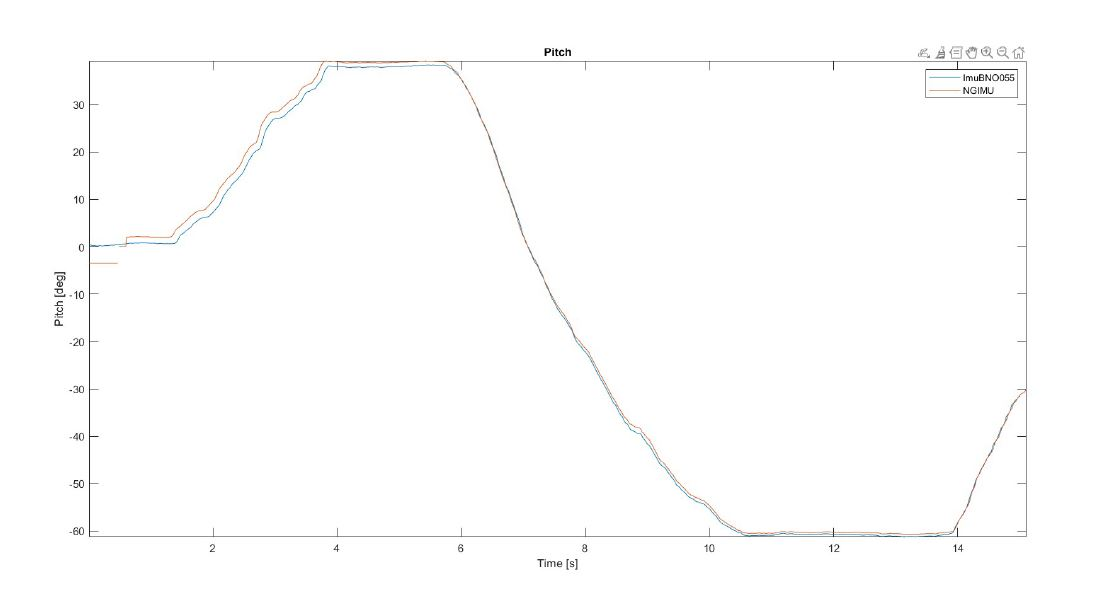
\includegraphics[width=0.8\textwidth,keepaspectratio]{figures/grafico.JPG}
% \caption{Esempio di grafico}
% \label{fig:grafico}
% \end{figure}
% \chapter{Test1}
% Per ogni test riportate: cosa state testando, in che condizioni si è svolto il test, riferimenti a video/file di log che consegnate insieme a relazione e codice, grafici dei risultati, commento dei risultati.

% \chapter{Test2}

% \newpage
% \addcontentsline{toc}{chapter}{Conclusioni e sviluppi futuri}
% \chapter*{Conclusioni e sviluppi futuri}
% Riassumere brevemente il lavoro svolto rispetto al task assegnato, evidenziando quali risultati sono stati raggiunti e quali no. Se ci sono aspetti del task non completati spiegare quali sono stati i problemi riscontrati in merito.\\
% Inserire considerazioni personali su possibili sviluppi futuri dell'attività svolta (idee per migliorarla che non avete avuto modo di sperimentare, aspetti che suggerite di approfondire, problemi da risolvere..).

% \addcontentsline{toc}{chapter}{Appendici}
% \appendix
% \chapter{Appendice1}
% Se necessario ricorrete alle appendici per spiegare le parti "di contorno" dell'attività svolta e/o ciò che non riuscite ad inserire nello schema generale dei capitoli della relazione (es acquisizione dei dati con Matlab).


% \bibliographystyle{ieeetr}
% \bibliography{bibl} 
\end{document}
